\setchapterstyle{lines}
\chapter{Double-Cascade Event Generation}
\labch{signal_simulation_appendix}


\section{Model-Independent Simulation Distributions} \labsec{model_independent_simulation_appendix}

\begin{figure*}[h]
    \centering
    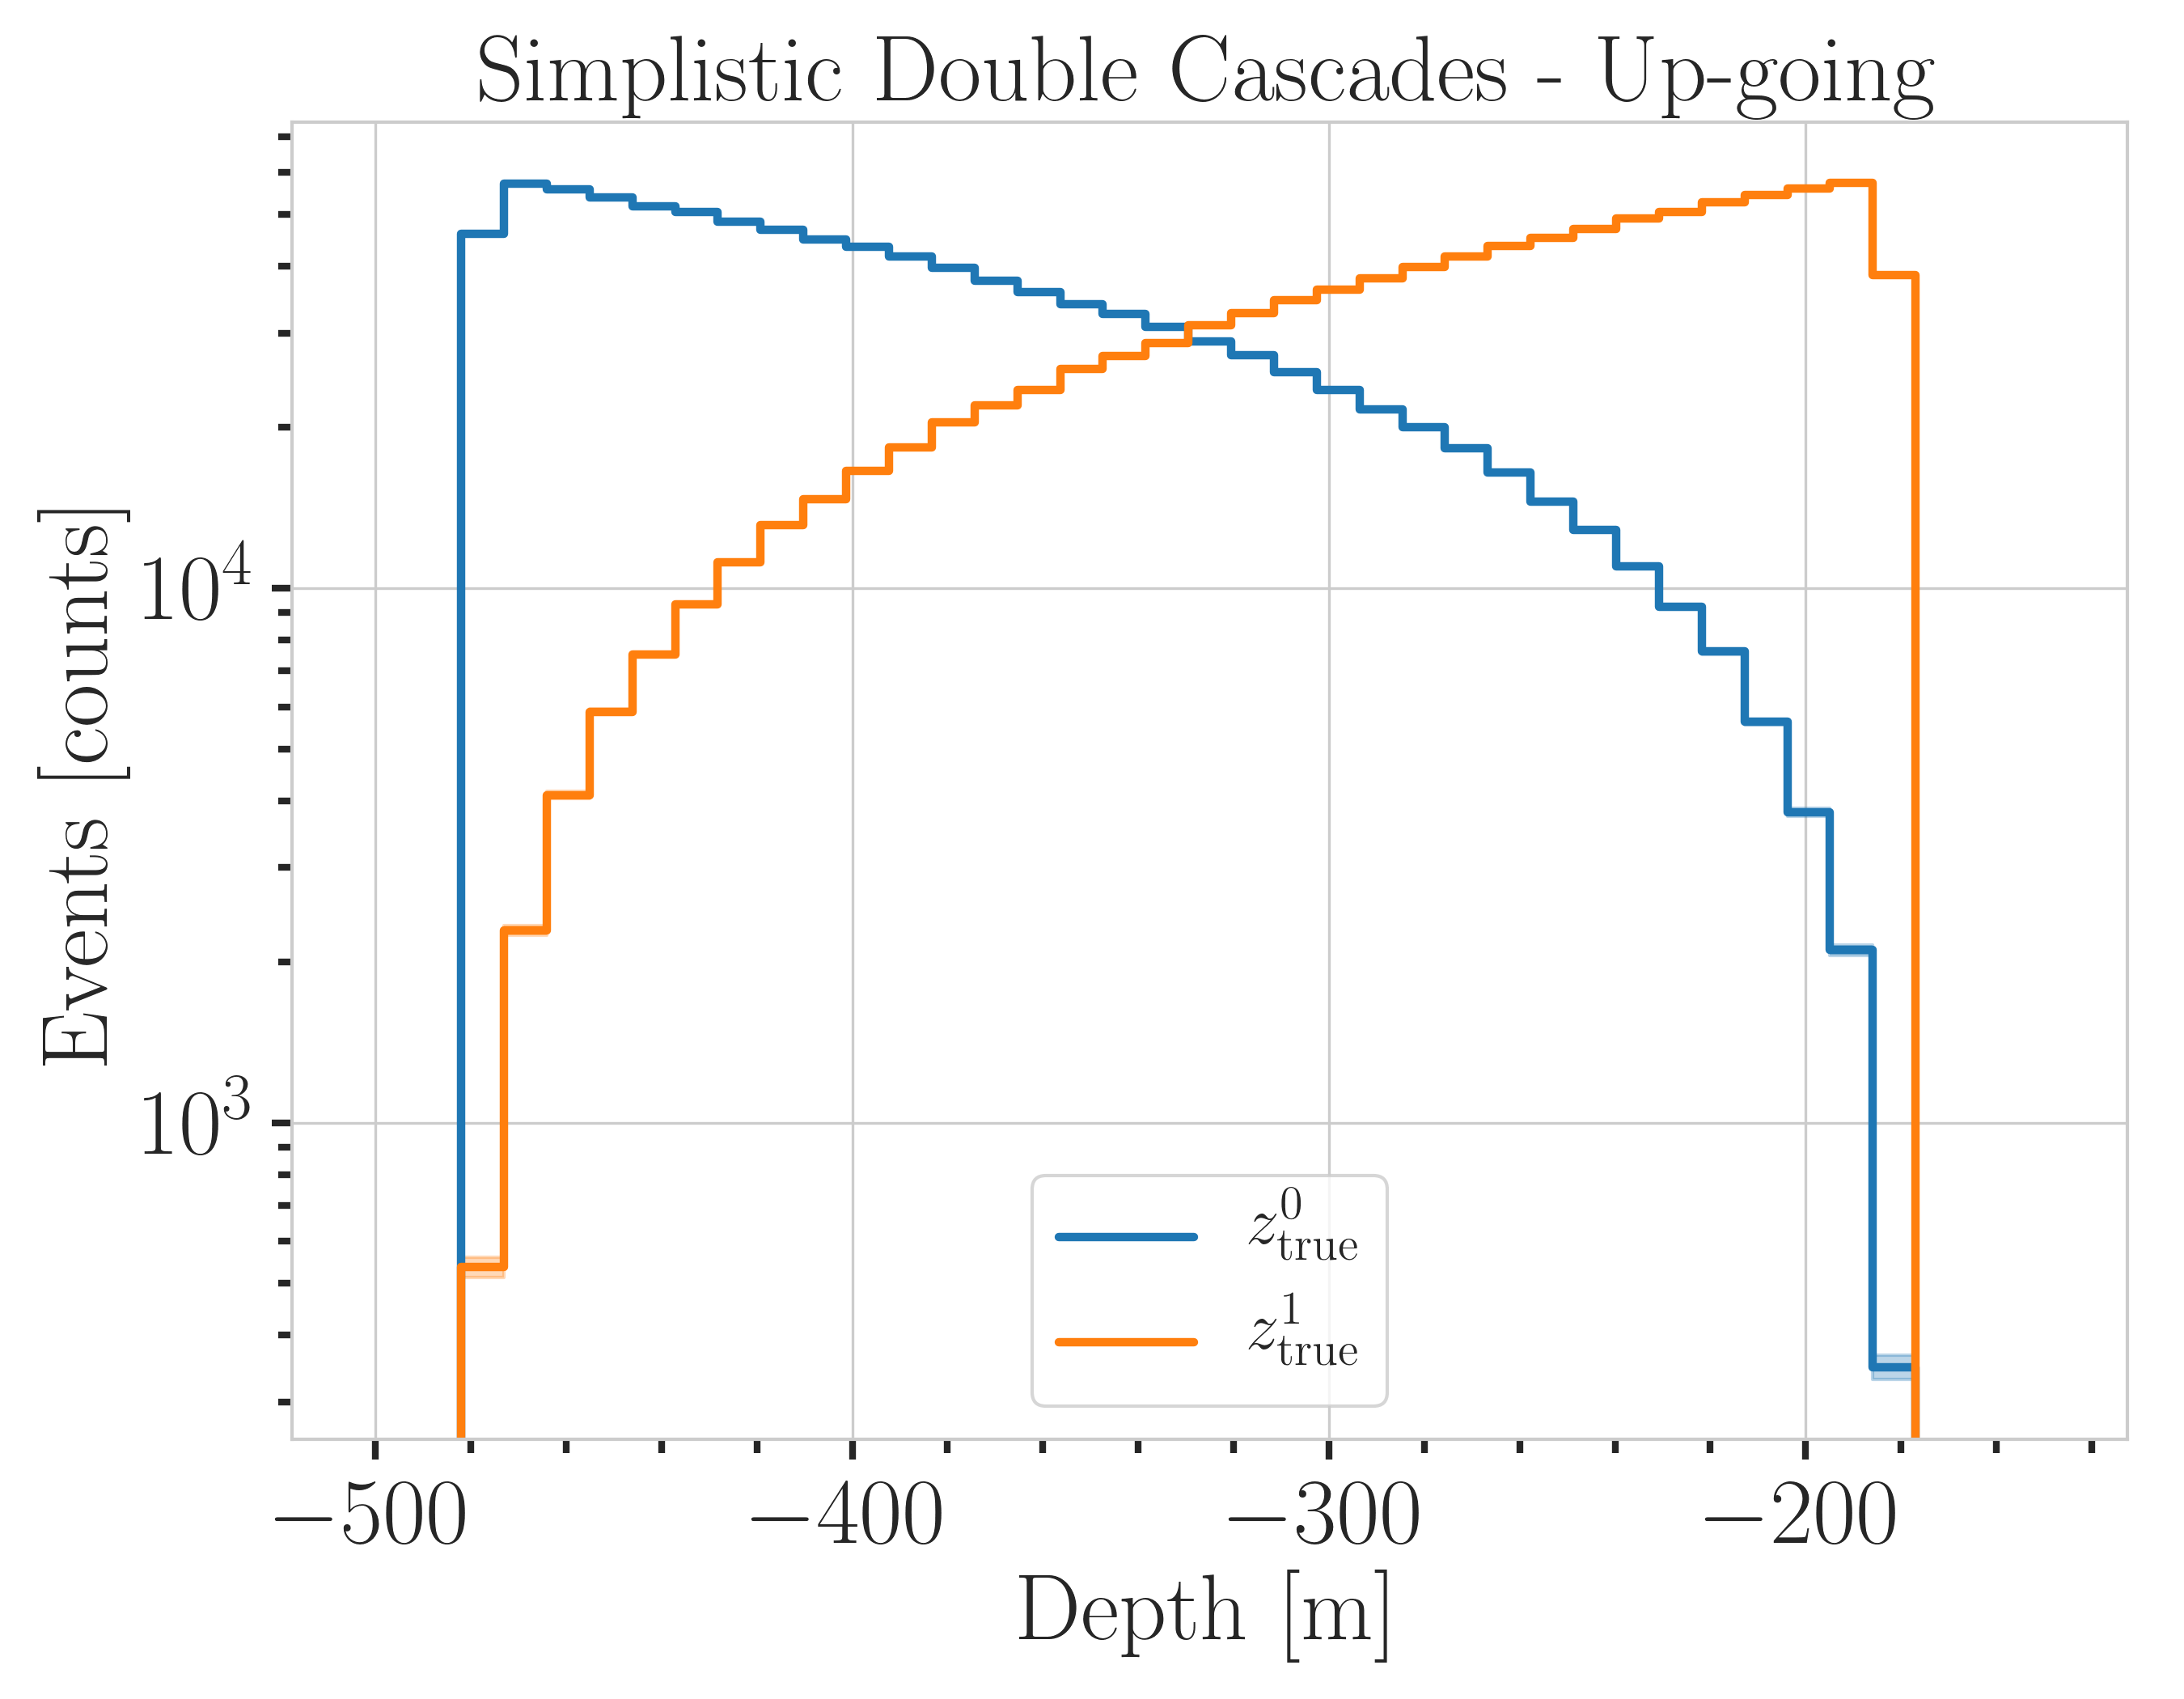
\includegraphics[width=0.49\linewidth]{figures/model_independent_simulation/gen_level/up_going_simplistic_1_d_distr_depth.png}
    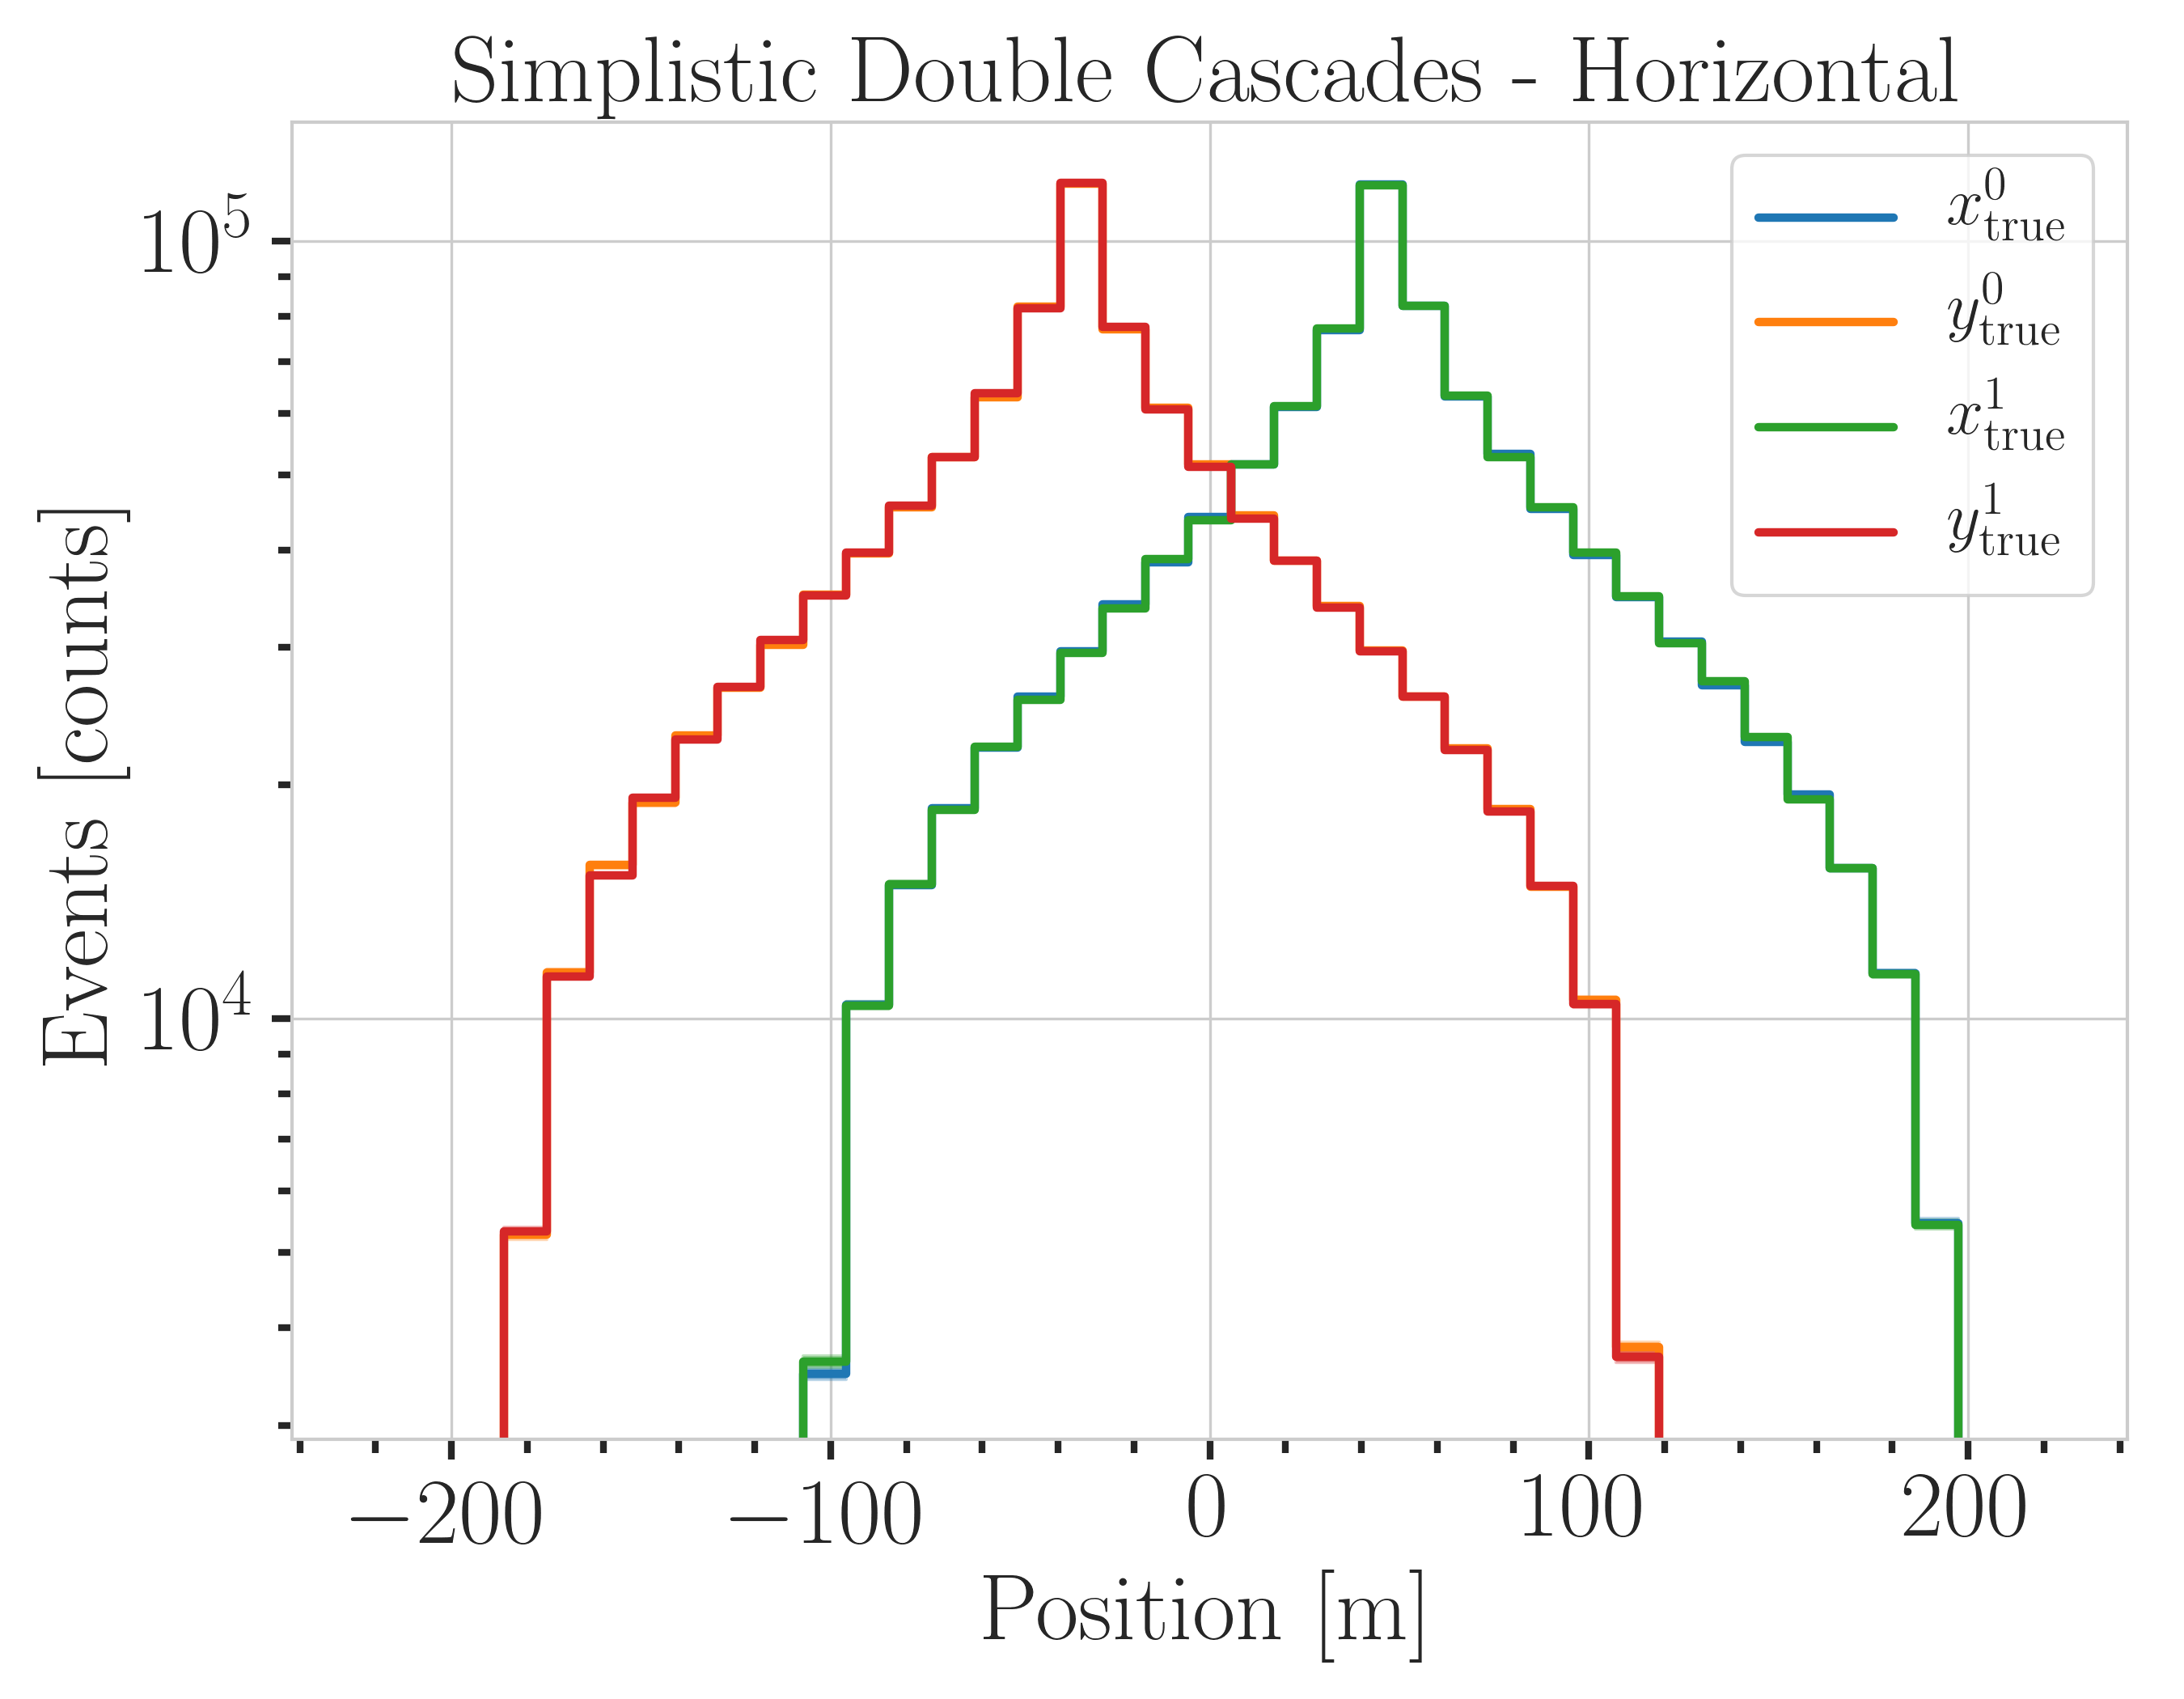
\includegraphics[width=0.49\linewidth]{figures/model_independent_simulation/gen_level/horizontal_simplistic_1_d_distr_position.png}
    \caption[Simplified model independent simulation generation level distributions]{Generation level distributions of the simplistic simulation sets. Vertical positions of the cascades in the up-going sample (left) and horizontal positions of the cascades in the horizontal sample (right).}
    \labfig{simplified_gen_distris_appendix}
\end{figure*}

\begin{figure*}
    \centering
    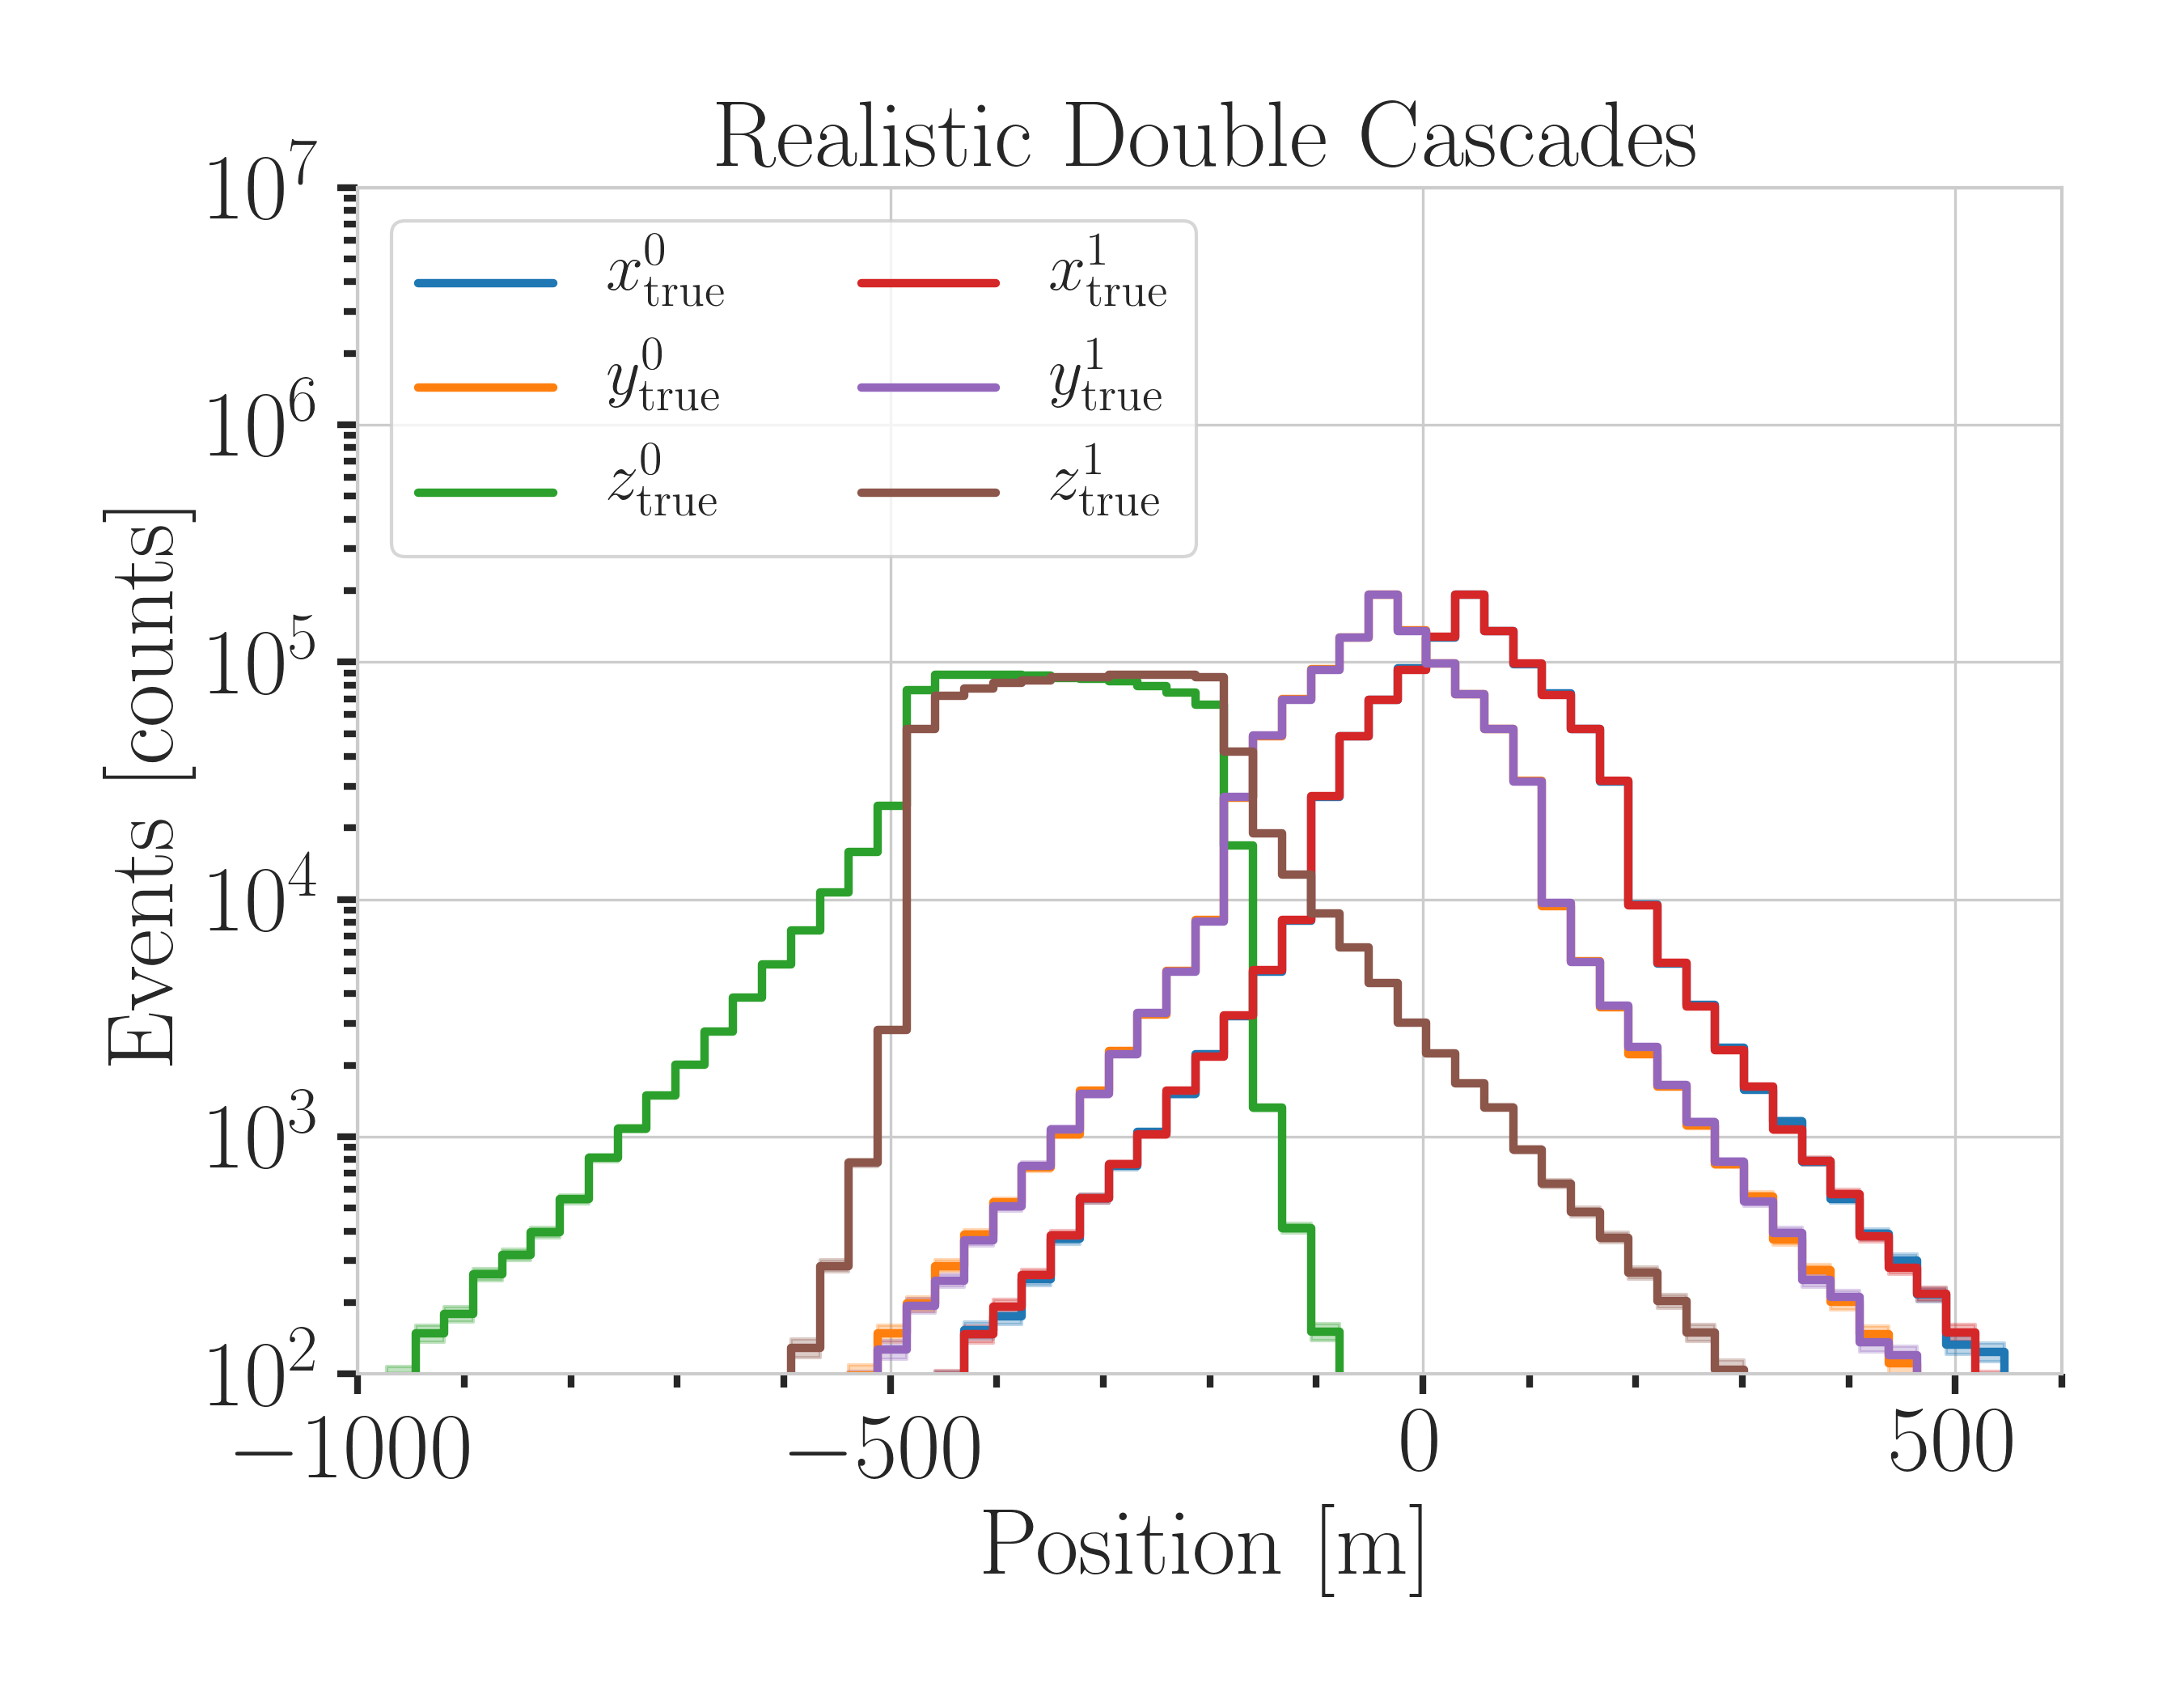
\includegraphics[width=0.49\linewidth]{figures/model_independent_simulation/gen_level/194603_gen_level_1_d_distr_cascade_positions.png}
    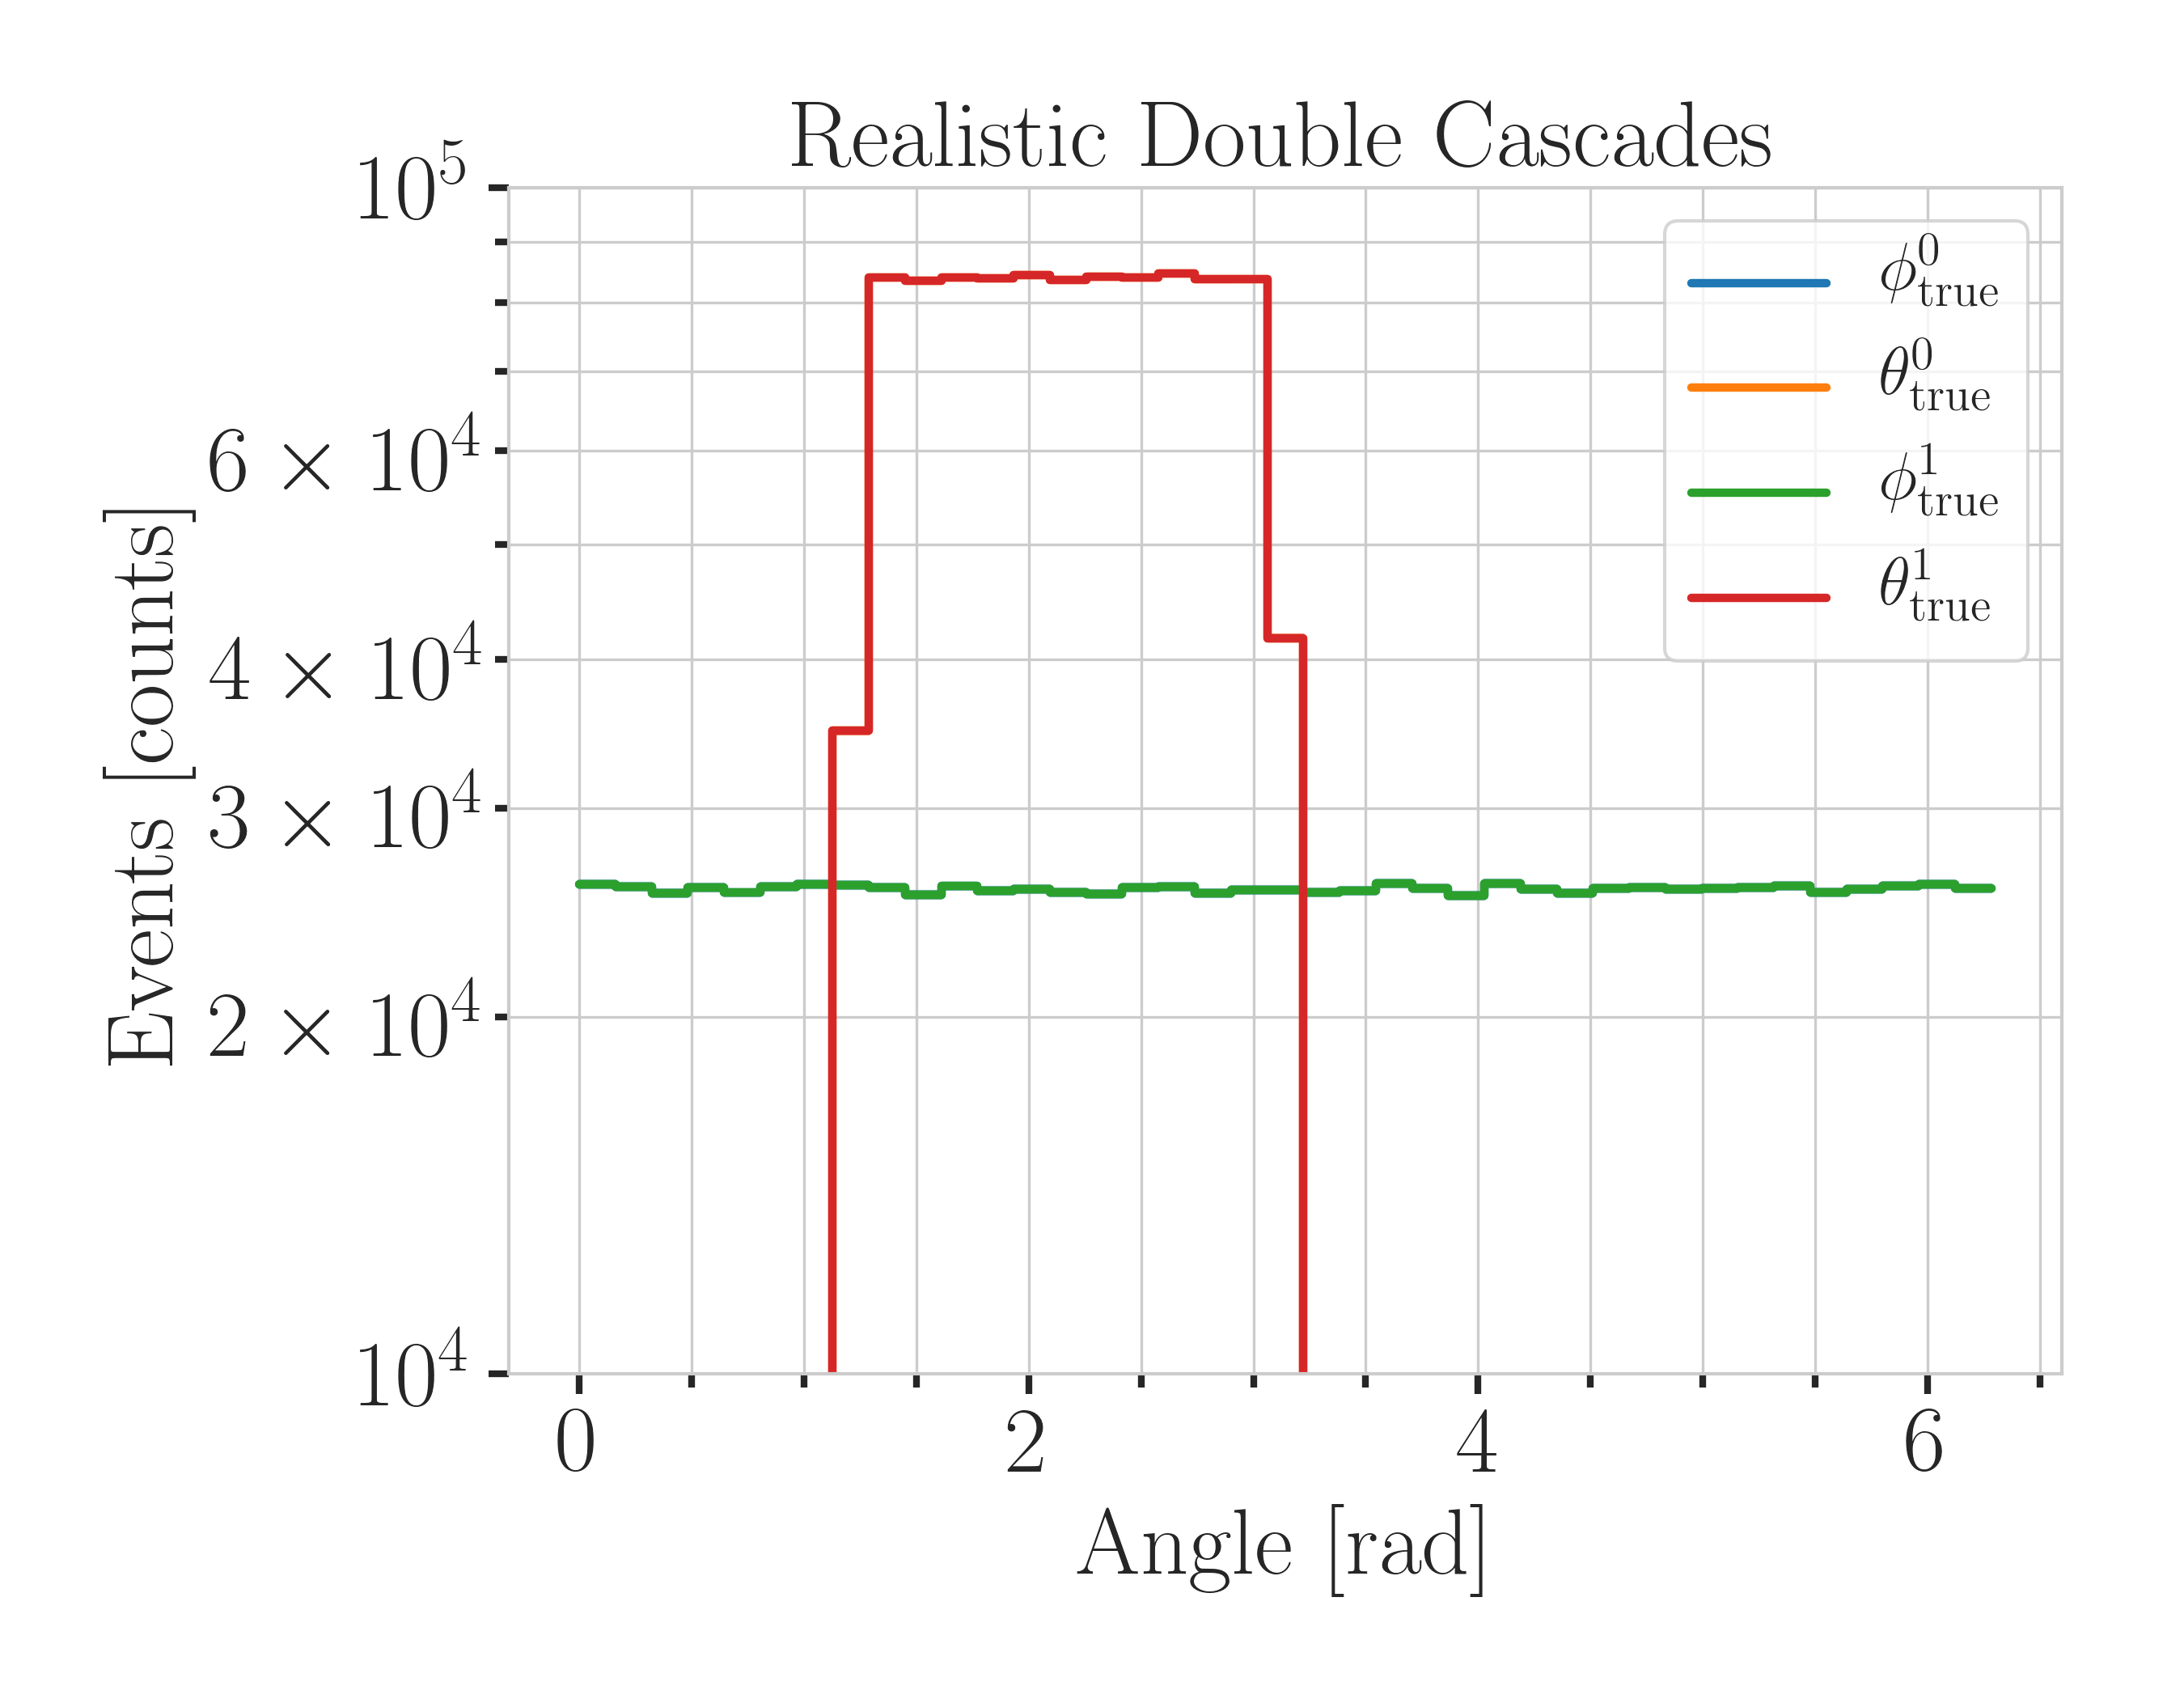
\includegraphics[width=0.49\linewidth]{figures/model_independent_simulation/gen_level/194603_gen_level_1_d_distr_cascade_directions.png}
    \caption[Realistic model independent simulation generation level distributions]{Generation level distributions of the realistic simulation set. Shown are the cascade $x, y, z$ positions (left) and the cascade direction angles (right).}
    \labfig{realistic_gen_distris_appendix}
\end{figure*}


\section{Model-Dependent Simulation Distributions} \labsec{model_dependent_simulation_appendix}

\begin{figure*}[h]
    \centering
    \begin{subfigure}{0.49\linewidth}
        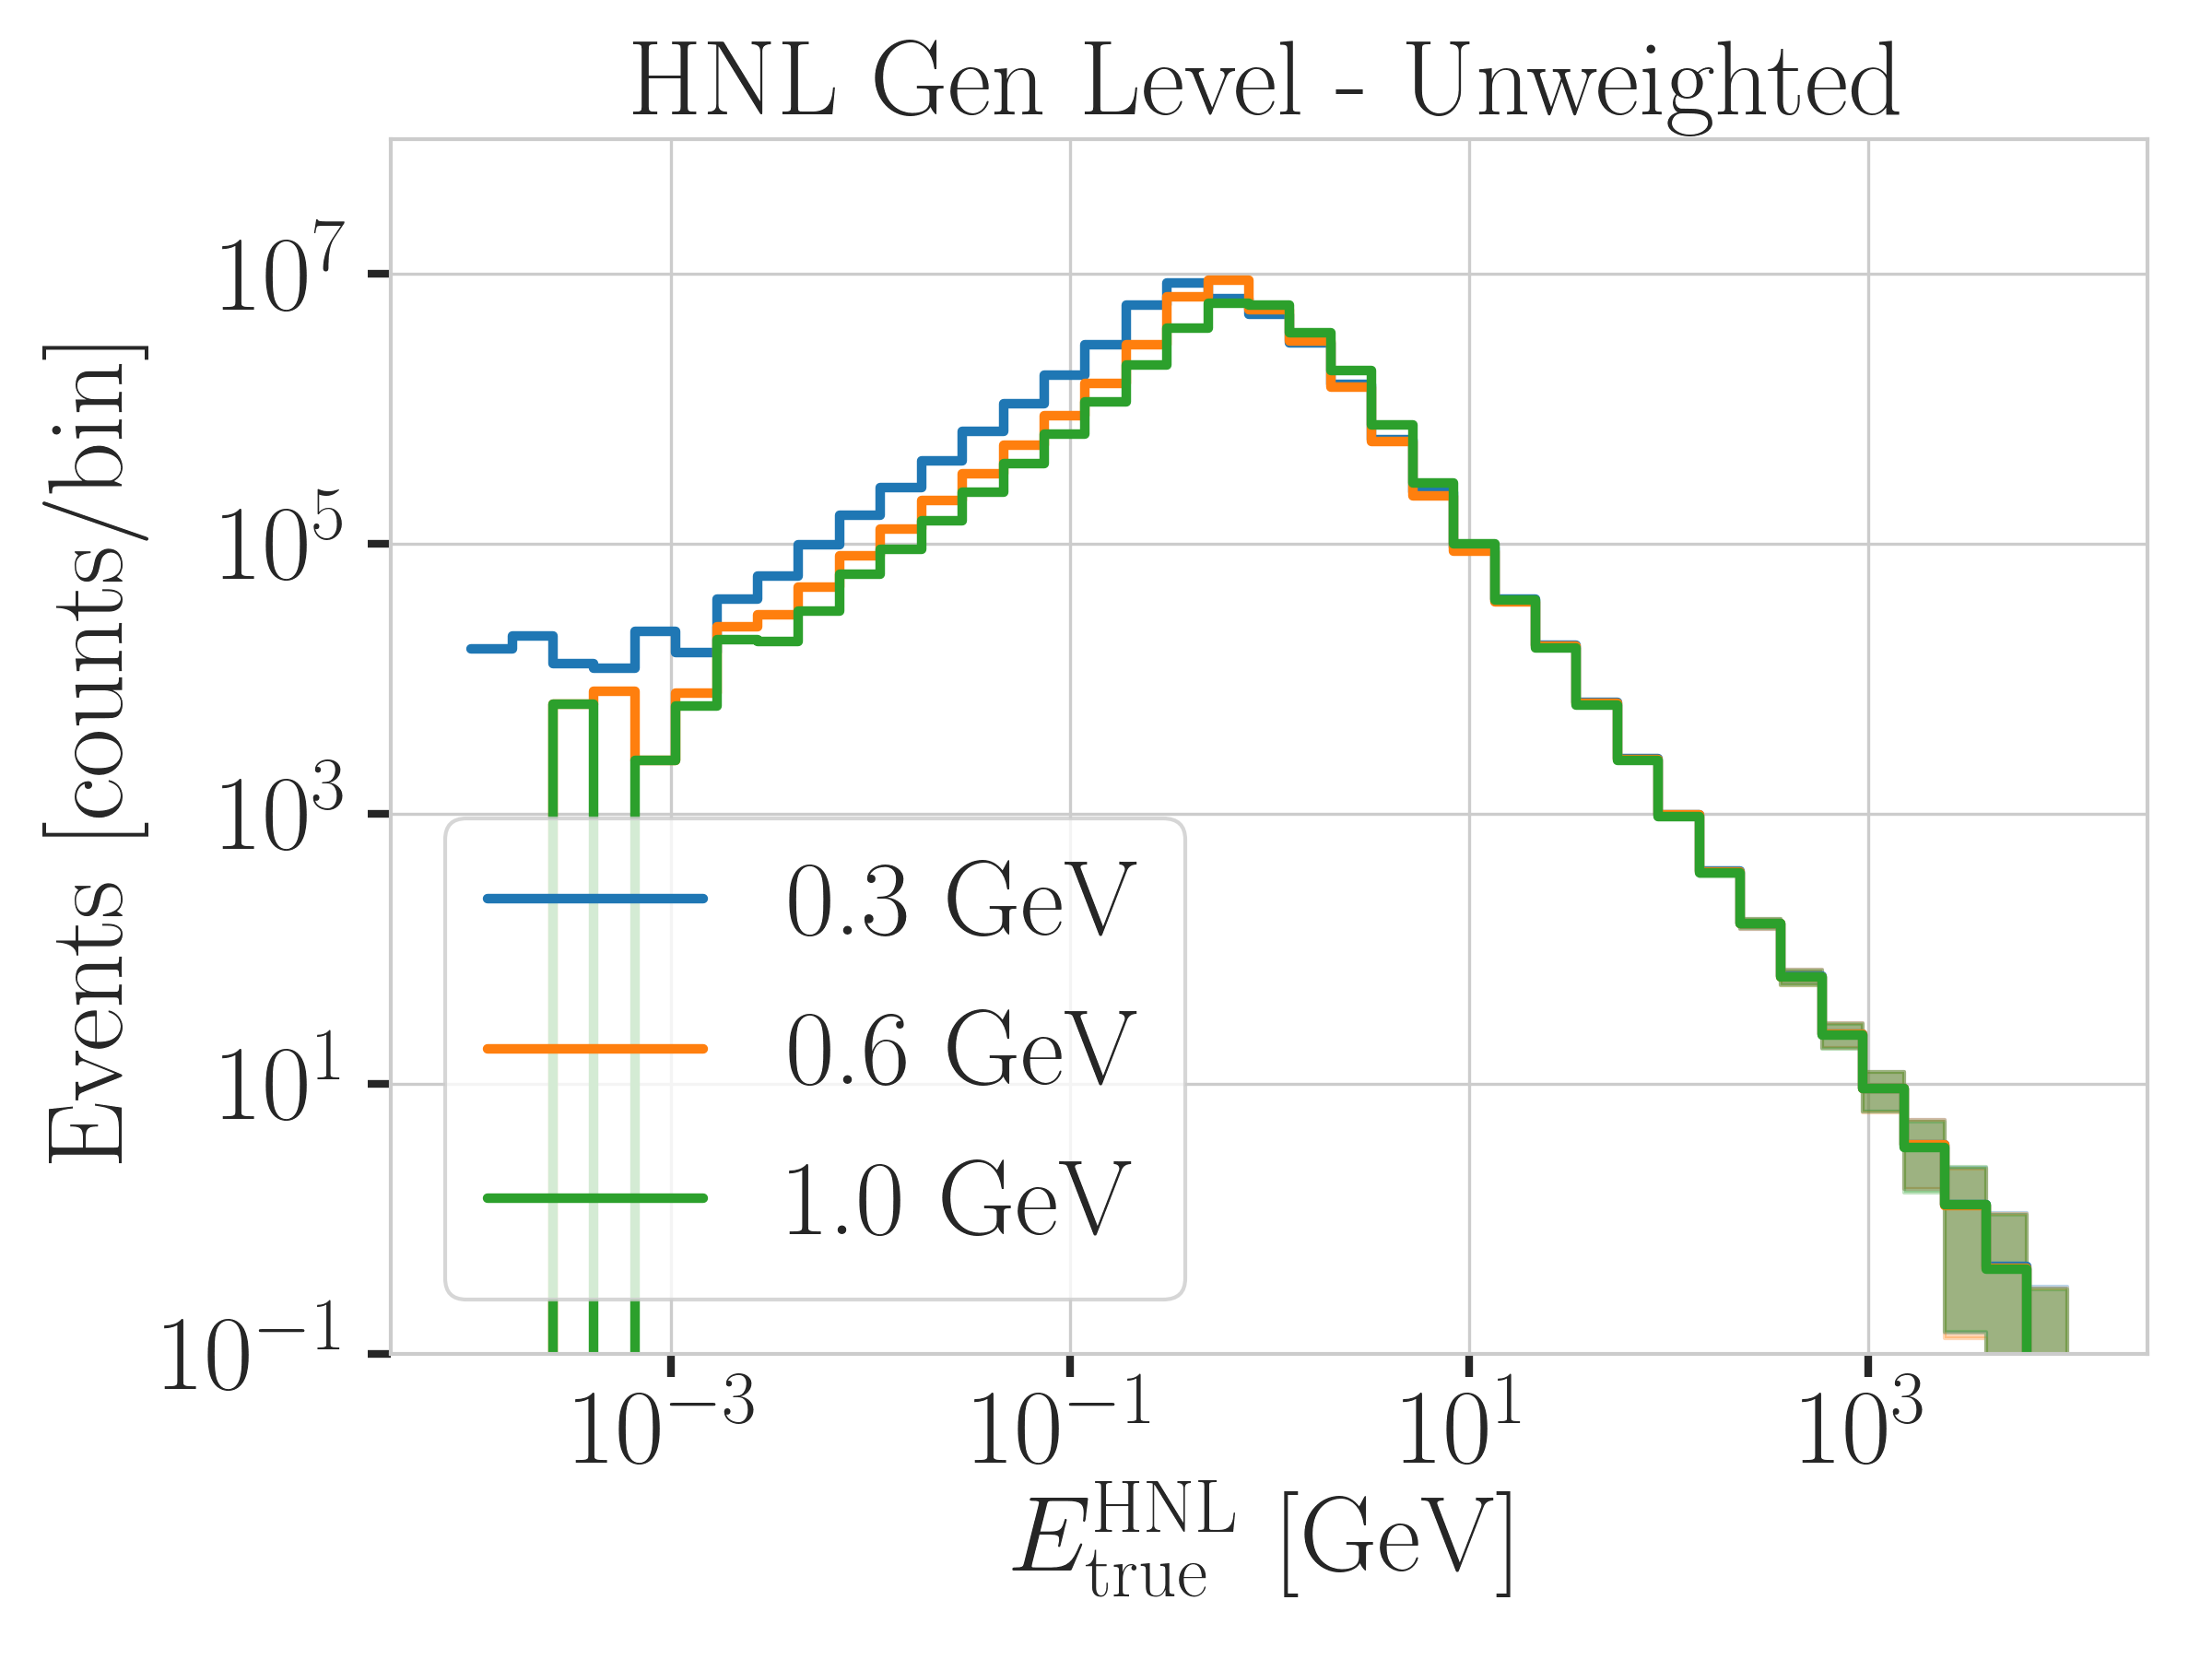
\includegraphics{figures/hnl_simulation/generation/1_d_distr_HNL_true_energy_gen_level_unweighted.png}
        \caption{HNL energy}
    \end{subfigure}
    \begin{subfigure}{0.49\linewidth}
        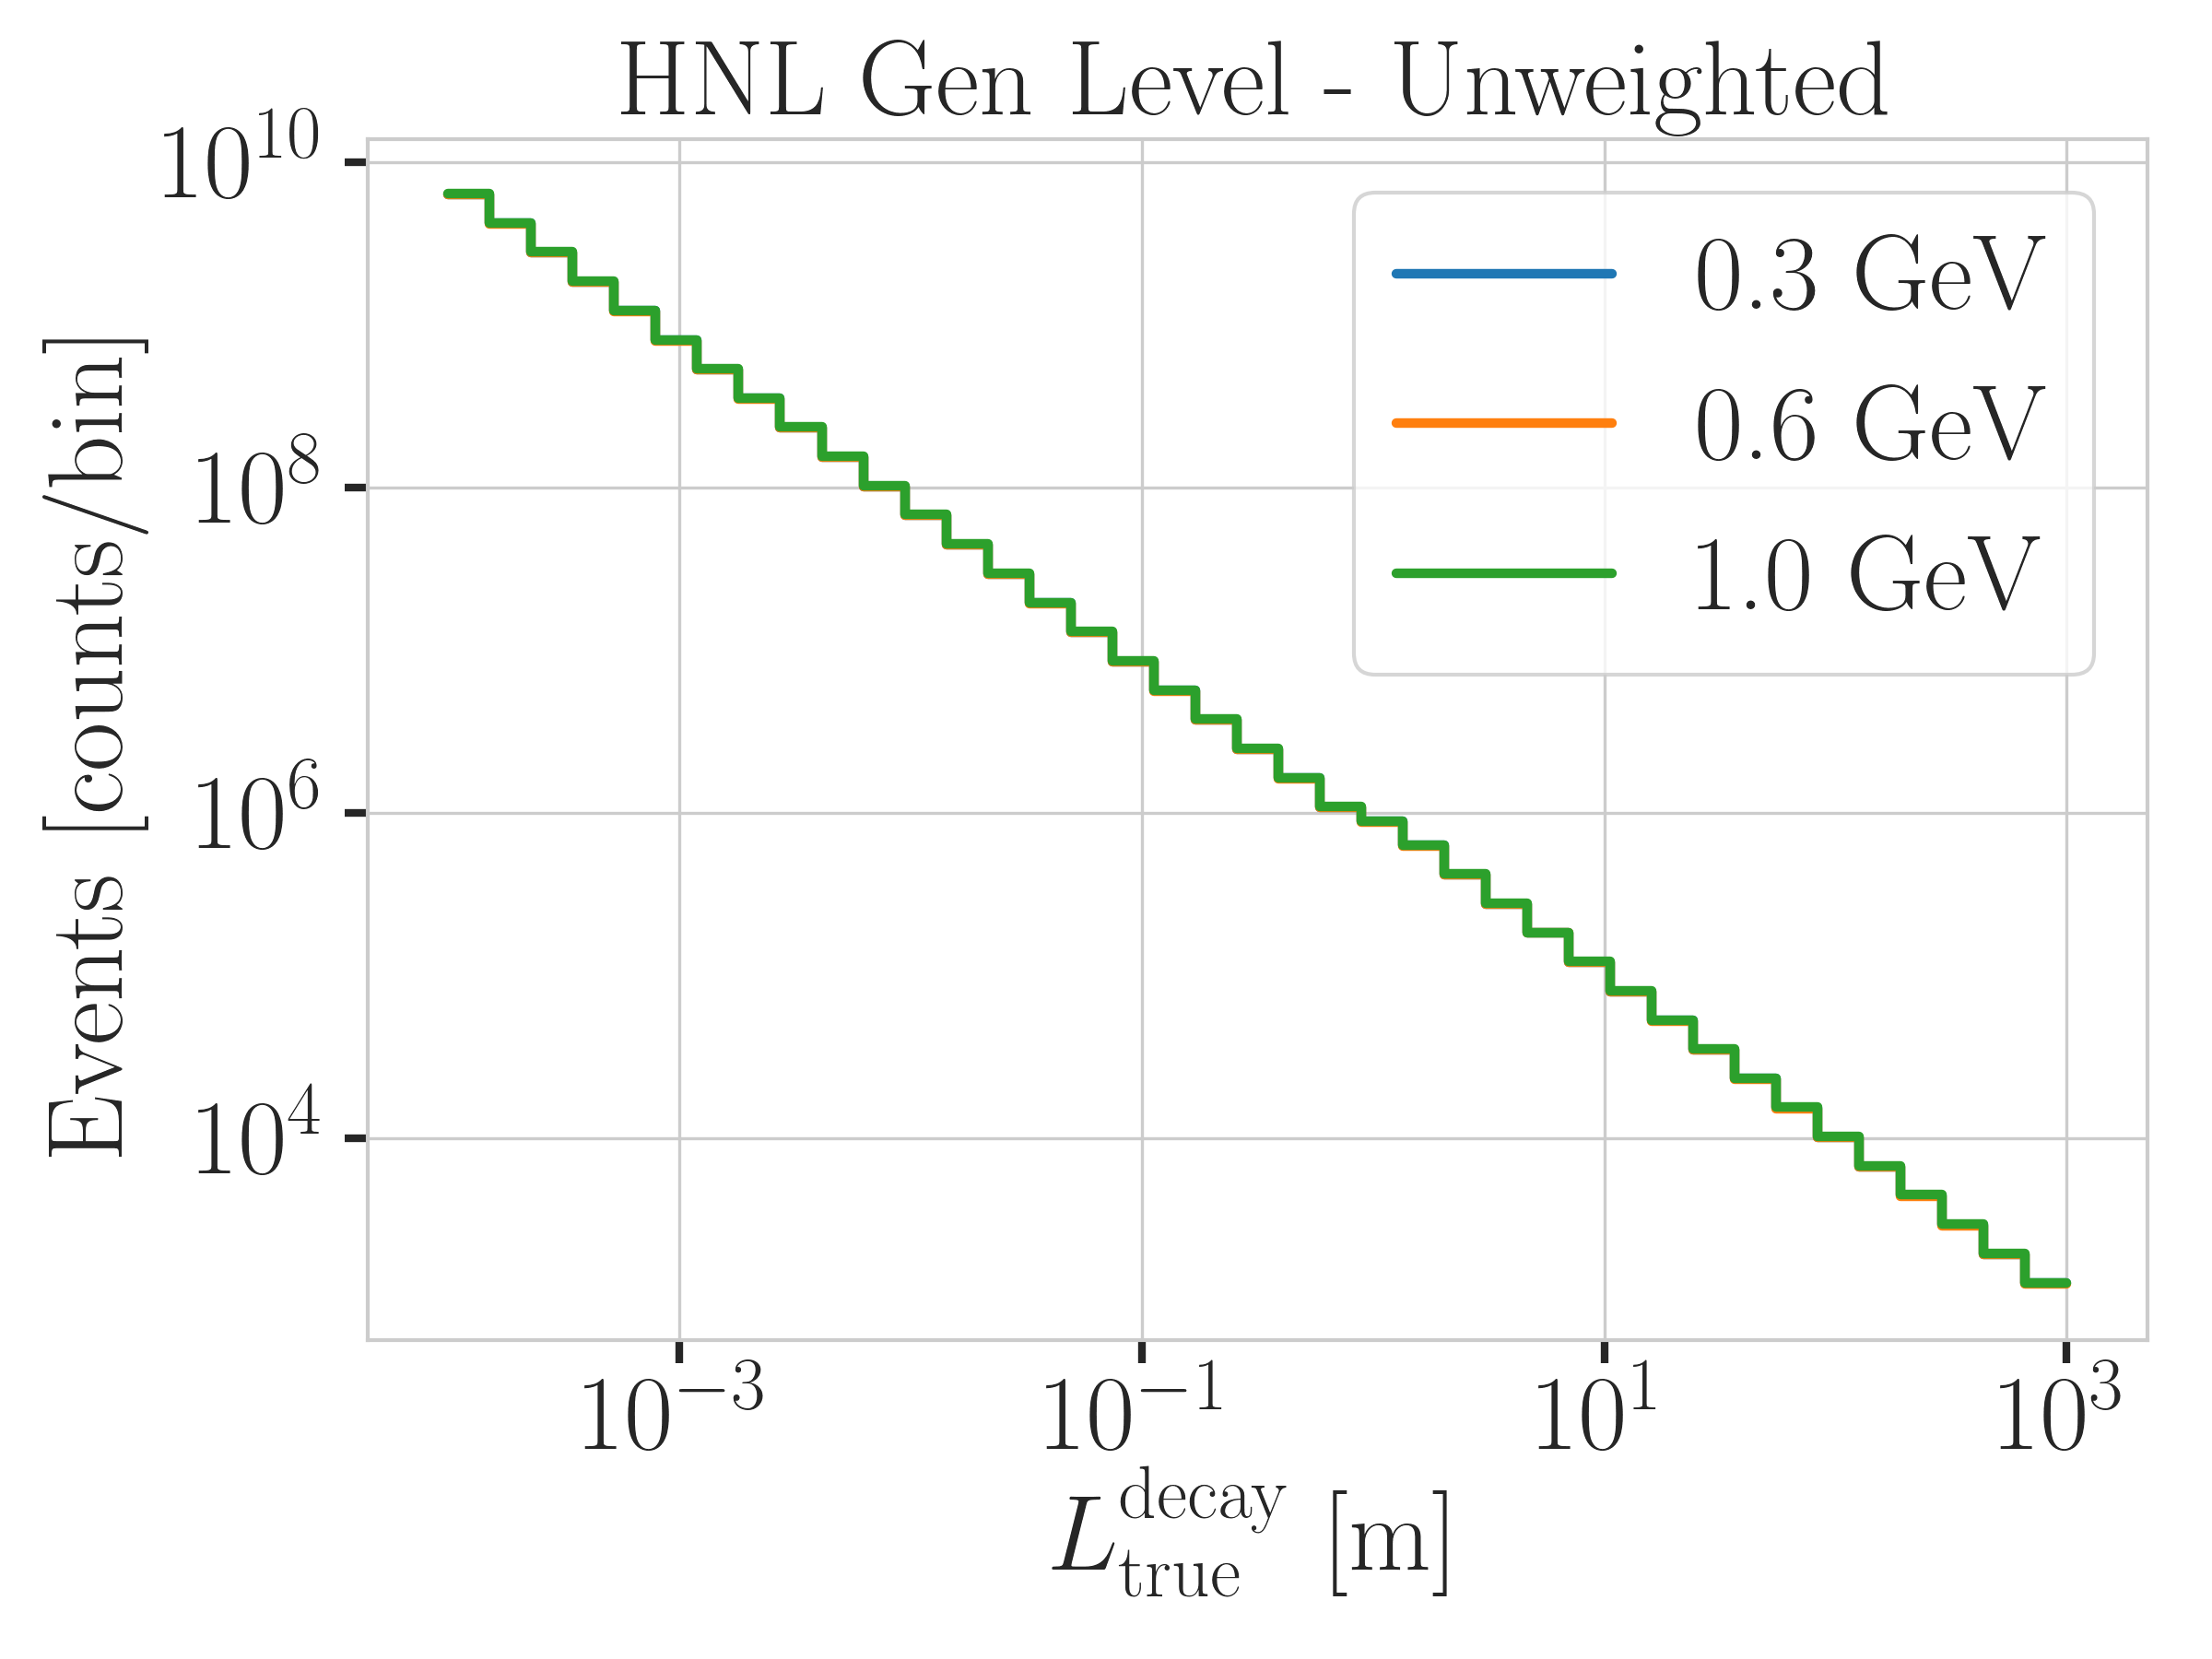
\includegraphics{figures/hnl_simulation/generation/1_d_distr_distance_gen_level_unweighted.png}
        \caption{Decay length}
    \end{subfigure}
    \begin{subfigure}{0.49\linewidth}
        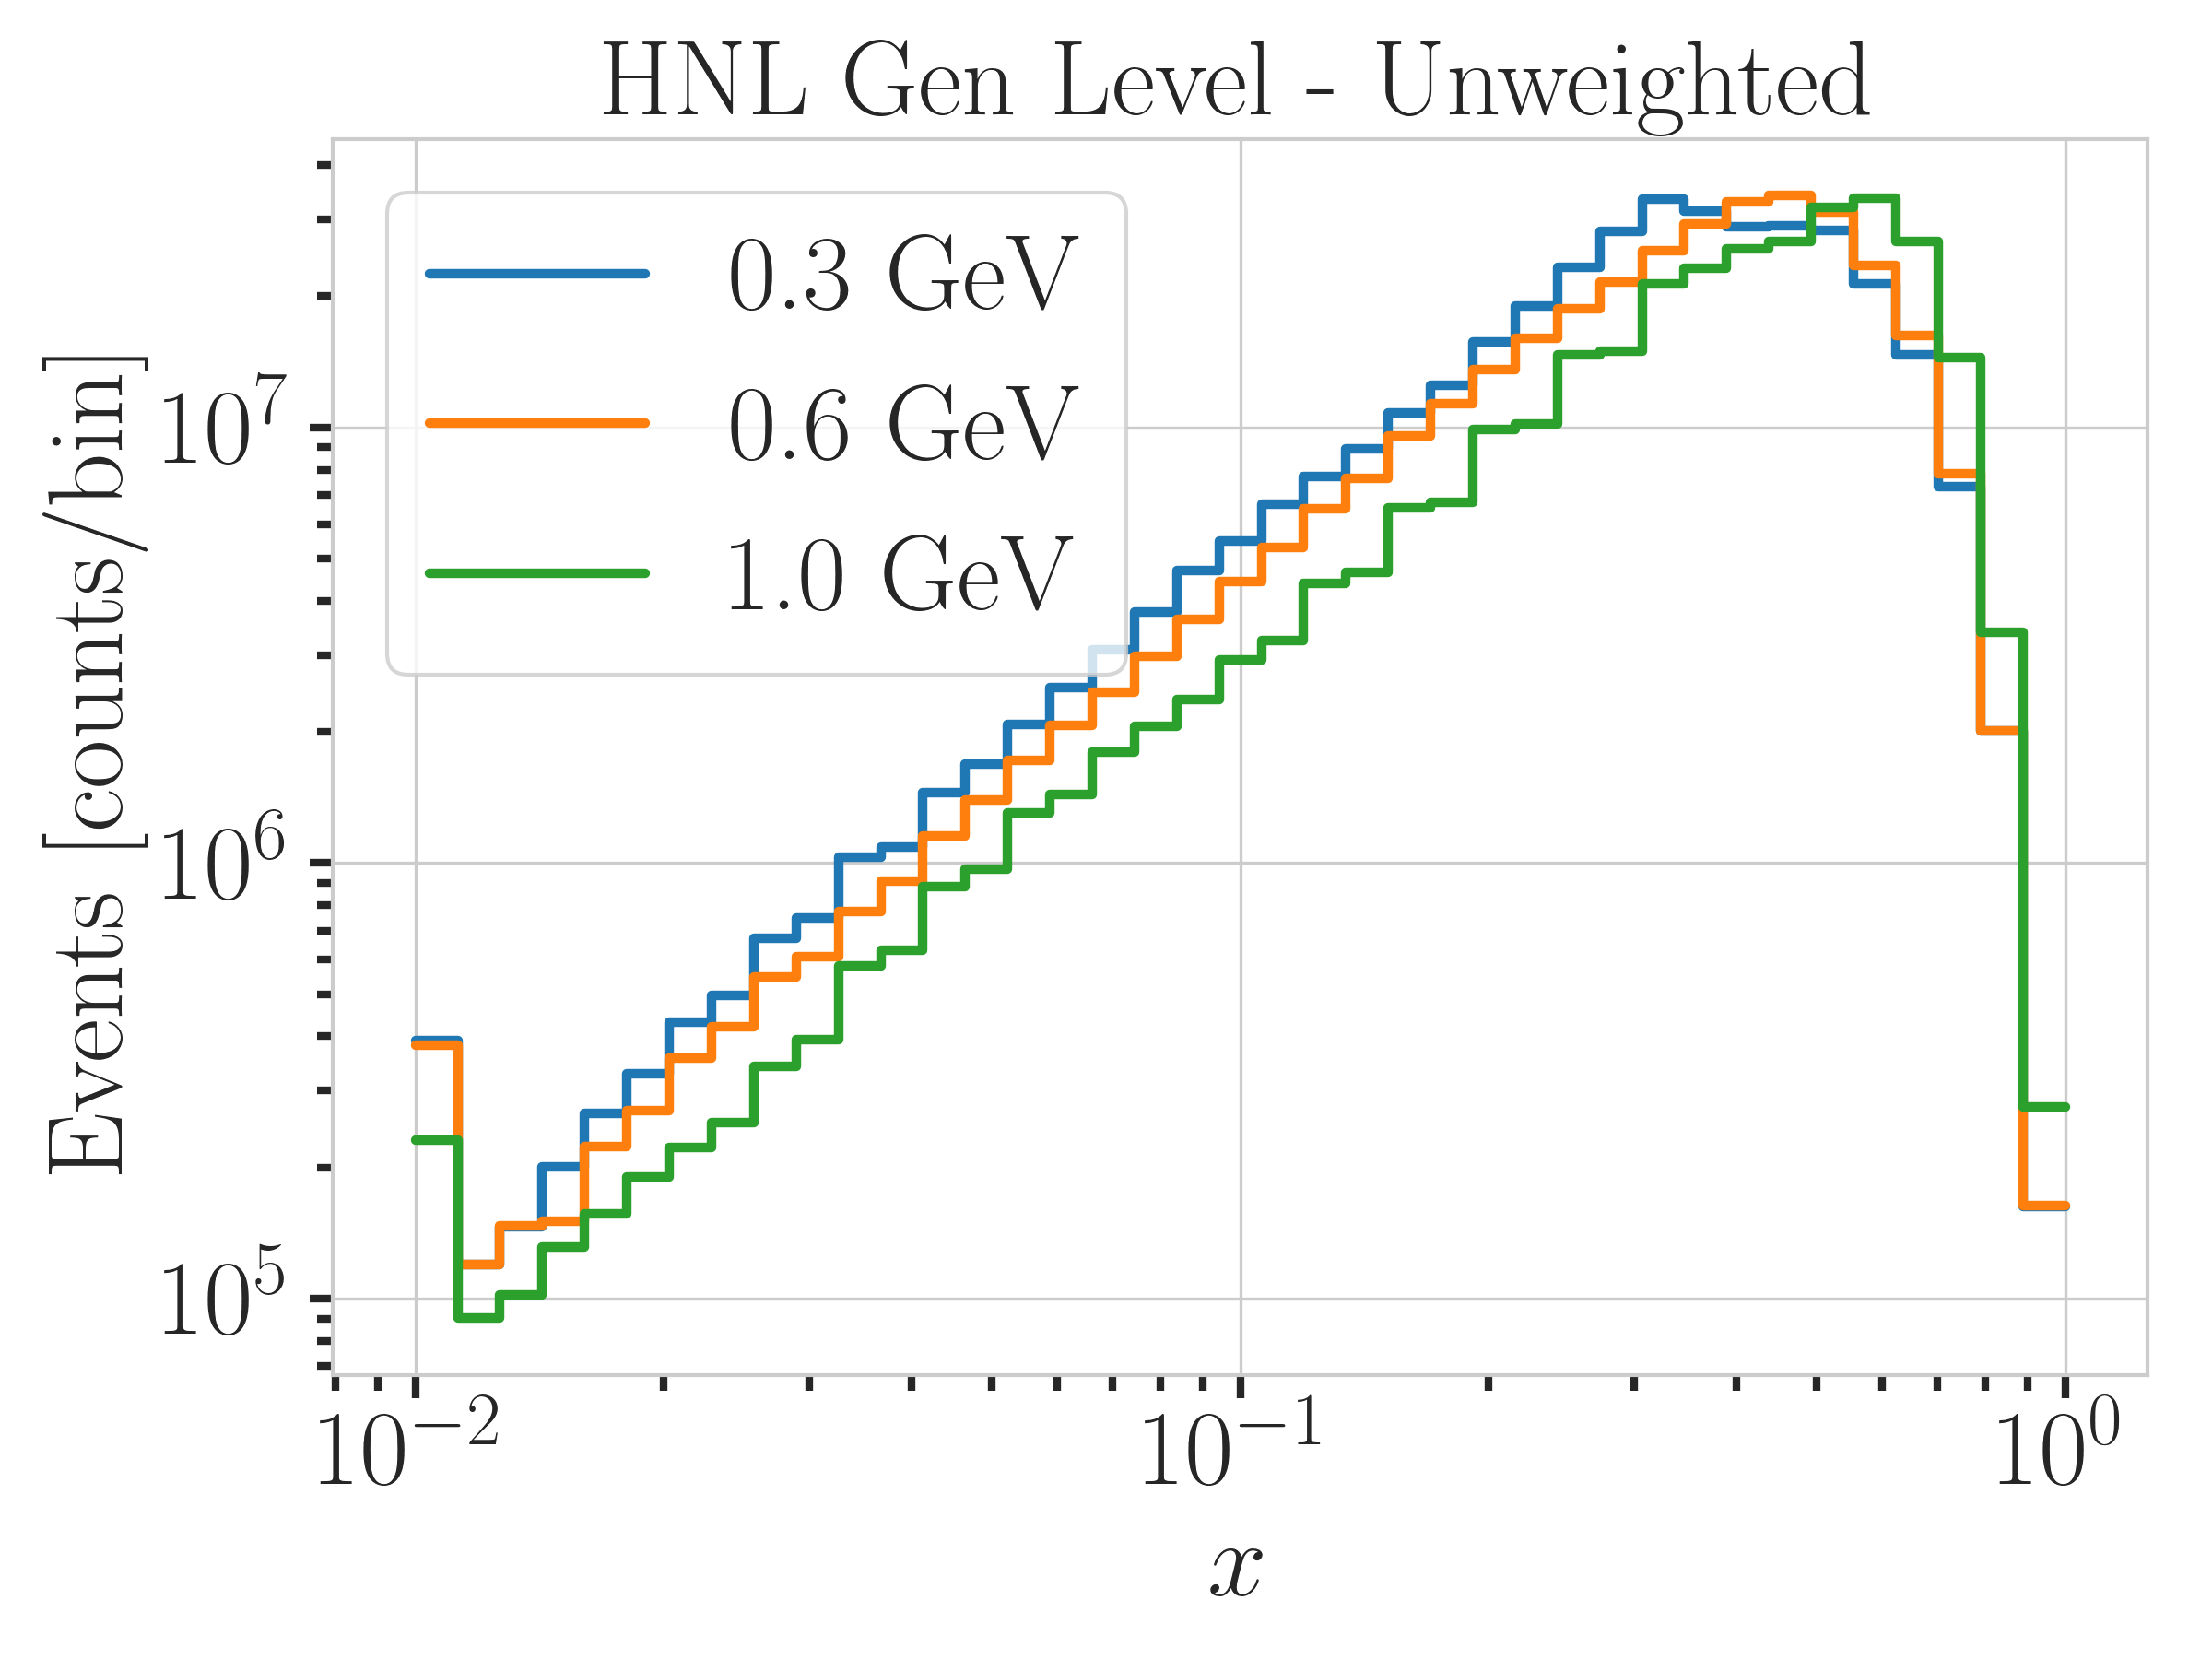
\includegraphics{figures/hnl_simulation/generation/1_d_distr_finalStateX_gen_level_unweighted.png}
        \caption{Bjorken x}
    \end{subfigure}
    \begin{subfigure}{0.49\linewidth}
    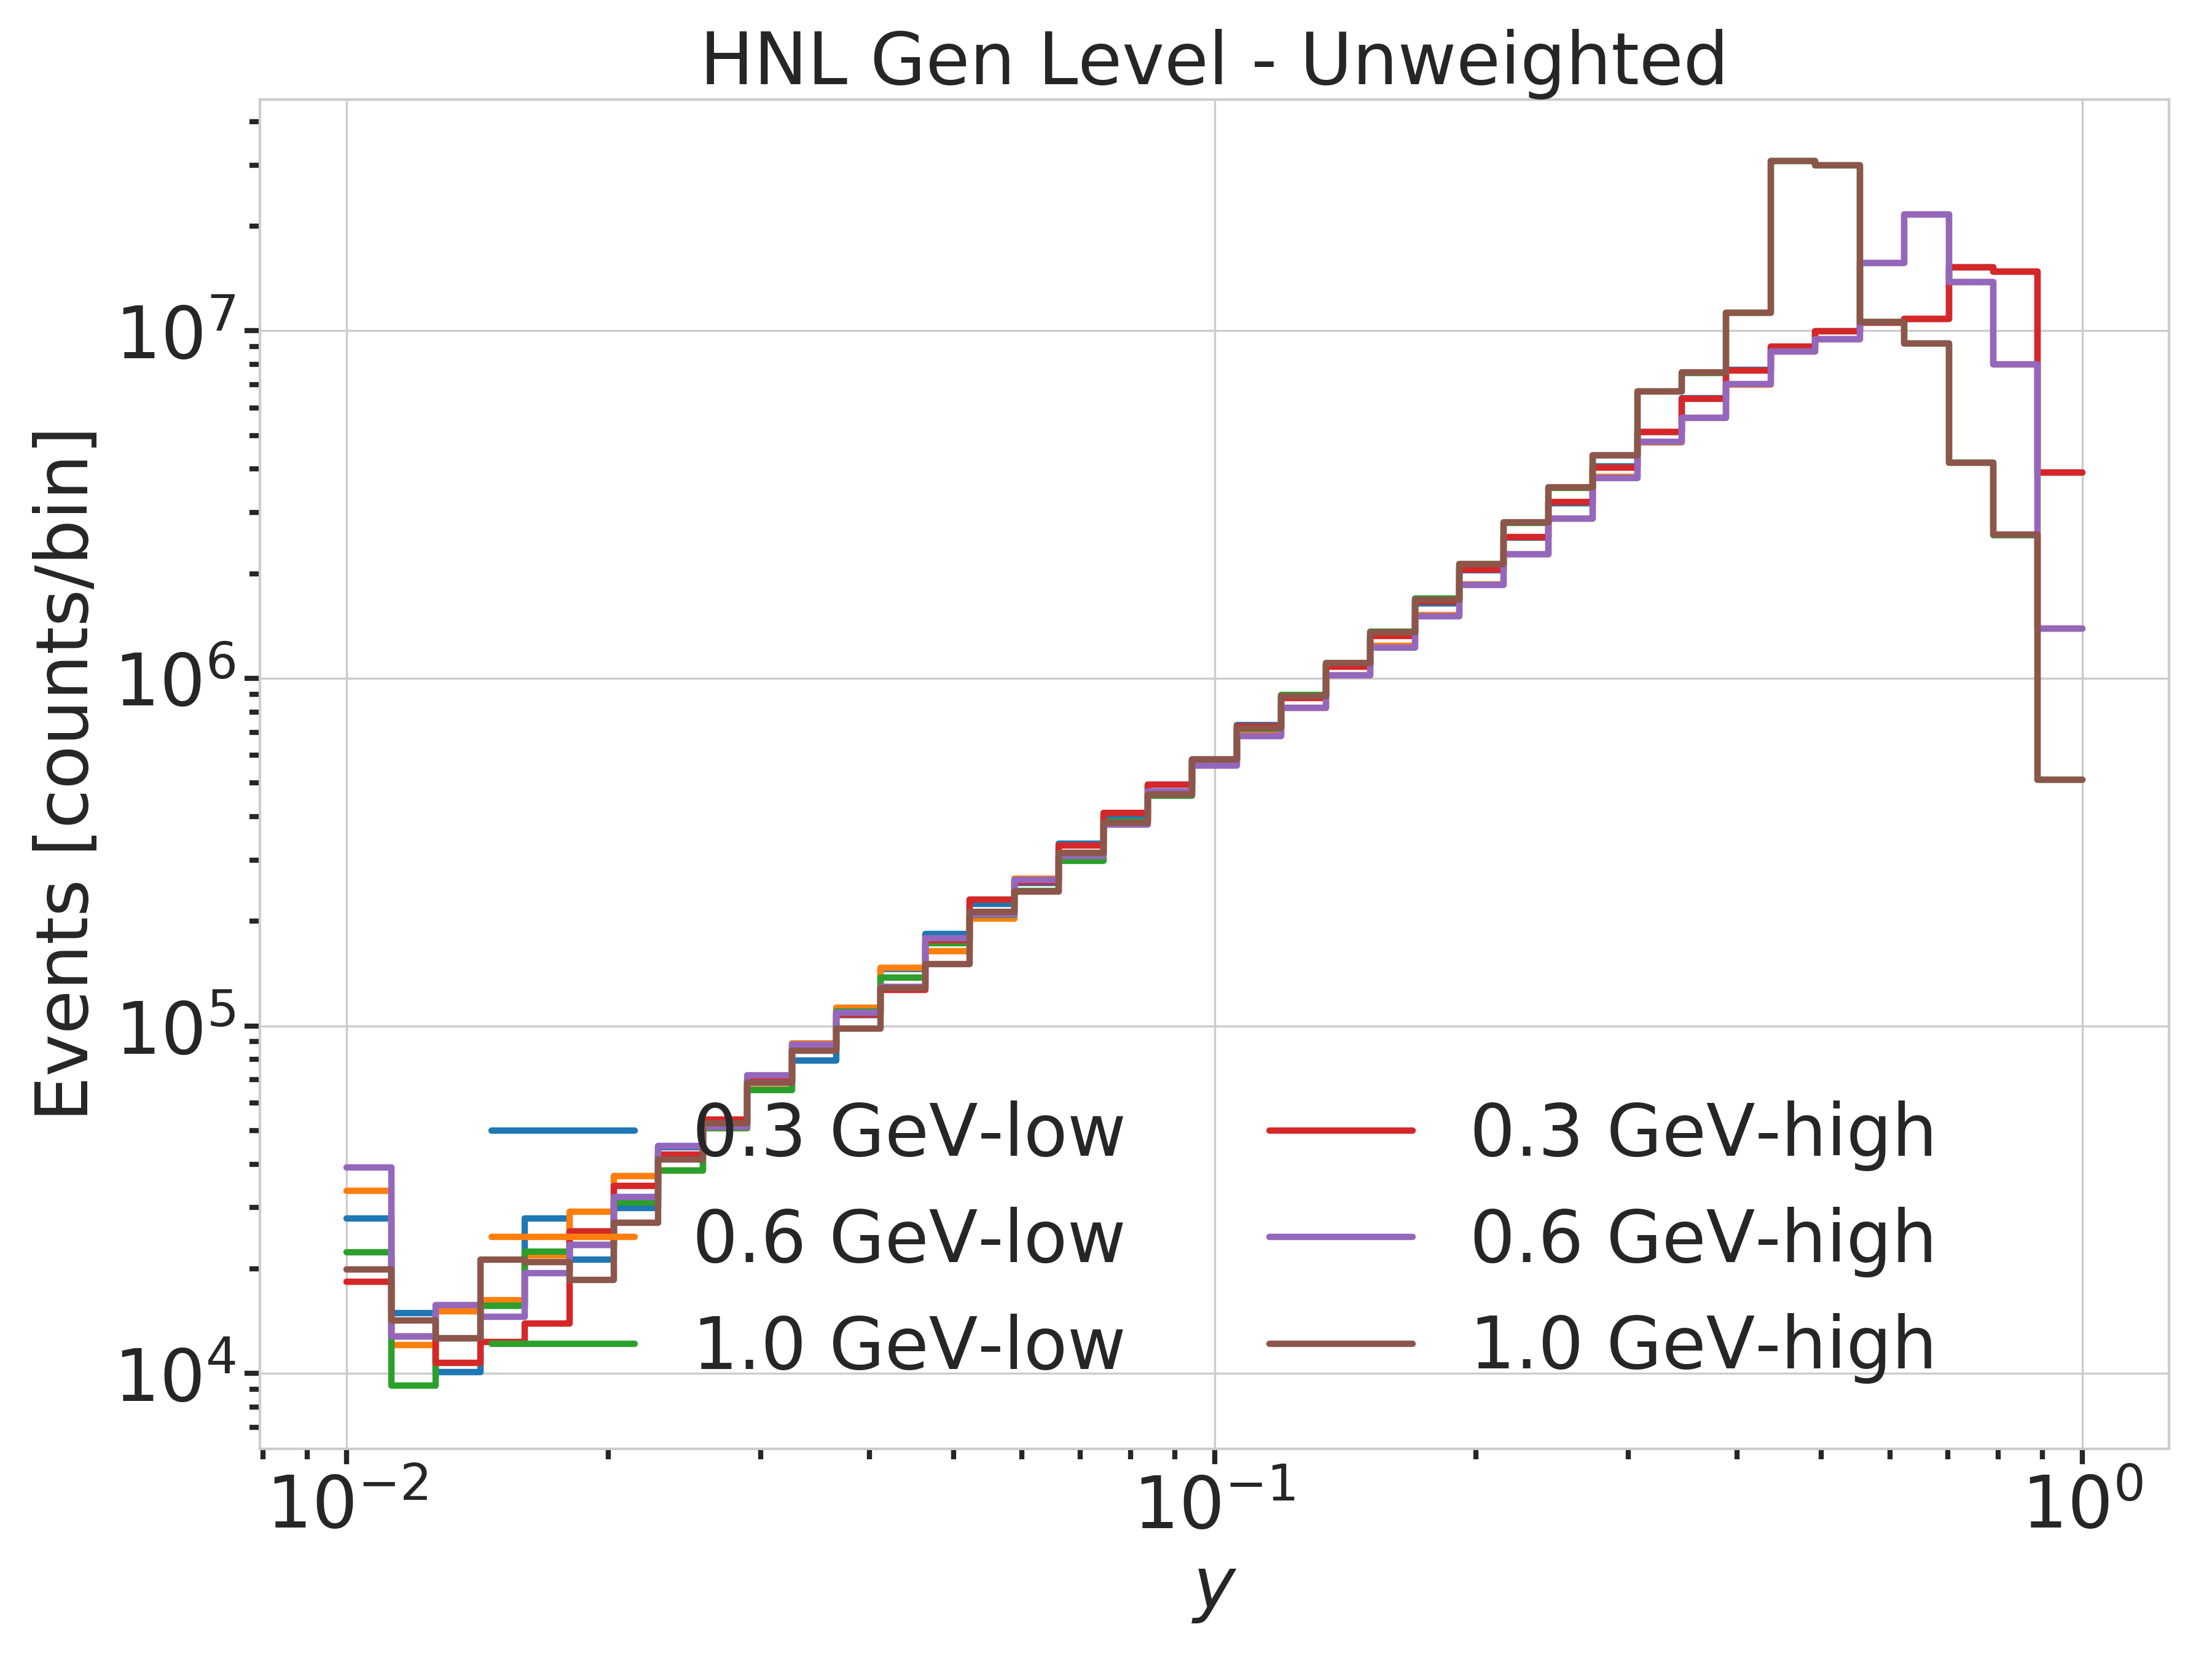
\includegraphics{figures/hnl_simulation/generation/1_d_distr_finalStateY_gen_level_unweighted.png}
        \caption{Bjorken y}
    \end{subfigure}
    \caption[Model dependent simulation generation level distributions]{Generation level distributions of the model dependent simulation.}
    \labfig{hnl_gen_distris_appendix}
\end{figure*}


\setchapterstyle{lines}
\chapter{Event Processing and Reconstruction}
\labch{processing_and_reconstruction_appendix}

\section{Double-Cascade Classifier Features} \labsec{dc_classifier_features_appendix}

\begin{figure*}[h]
    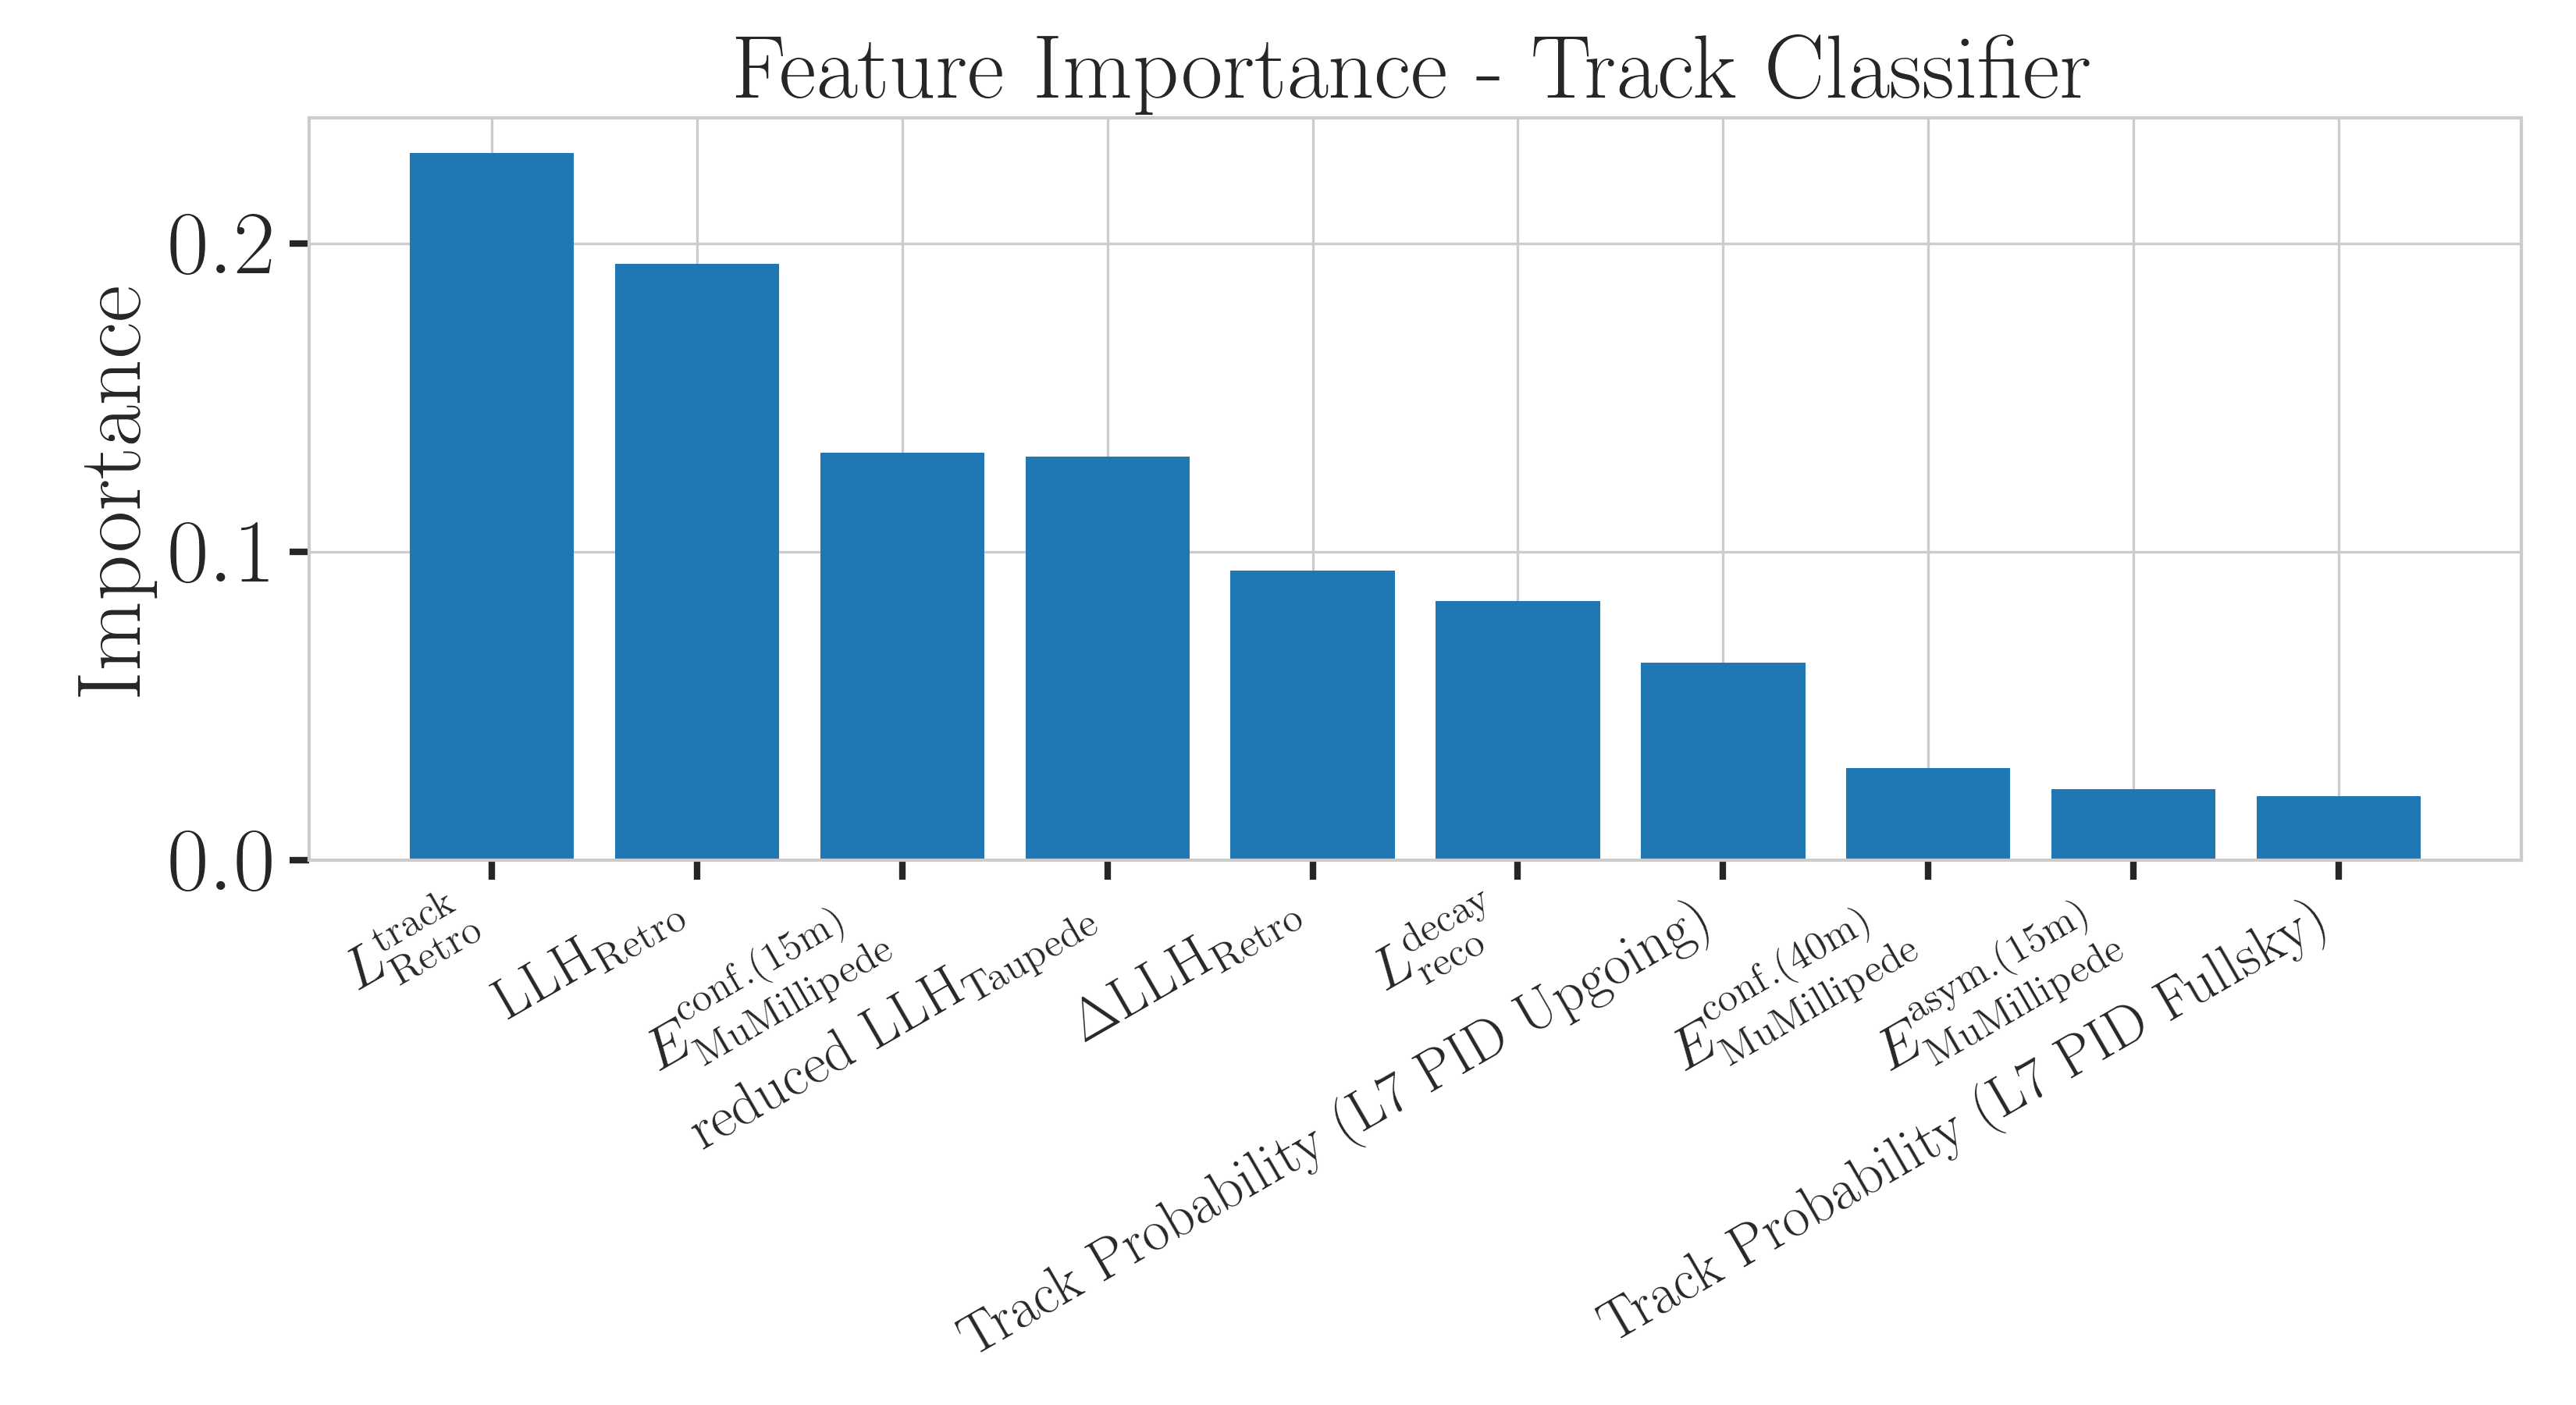
\includegraphics[width=0.8\linewidth]{figures/results/190607/classification/track_feature_importance.png}
    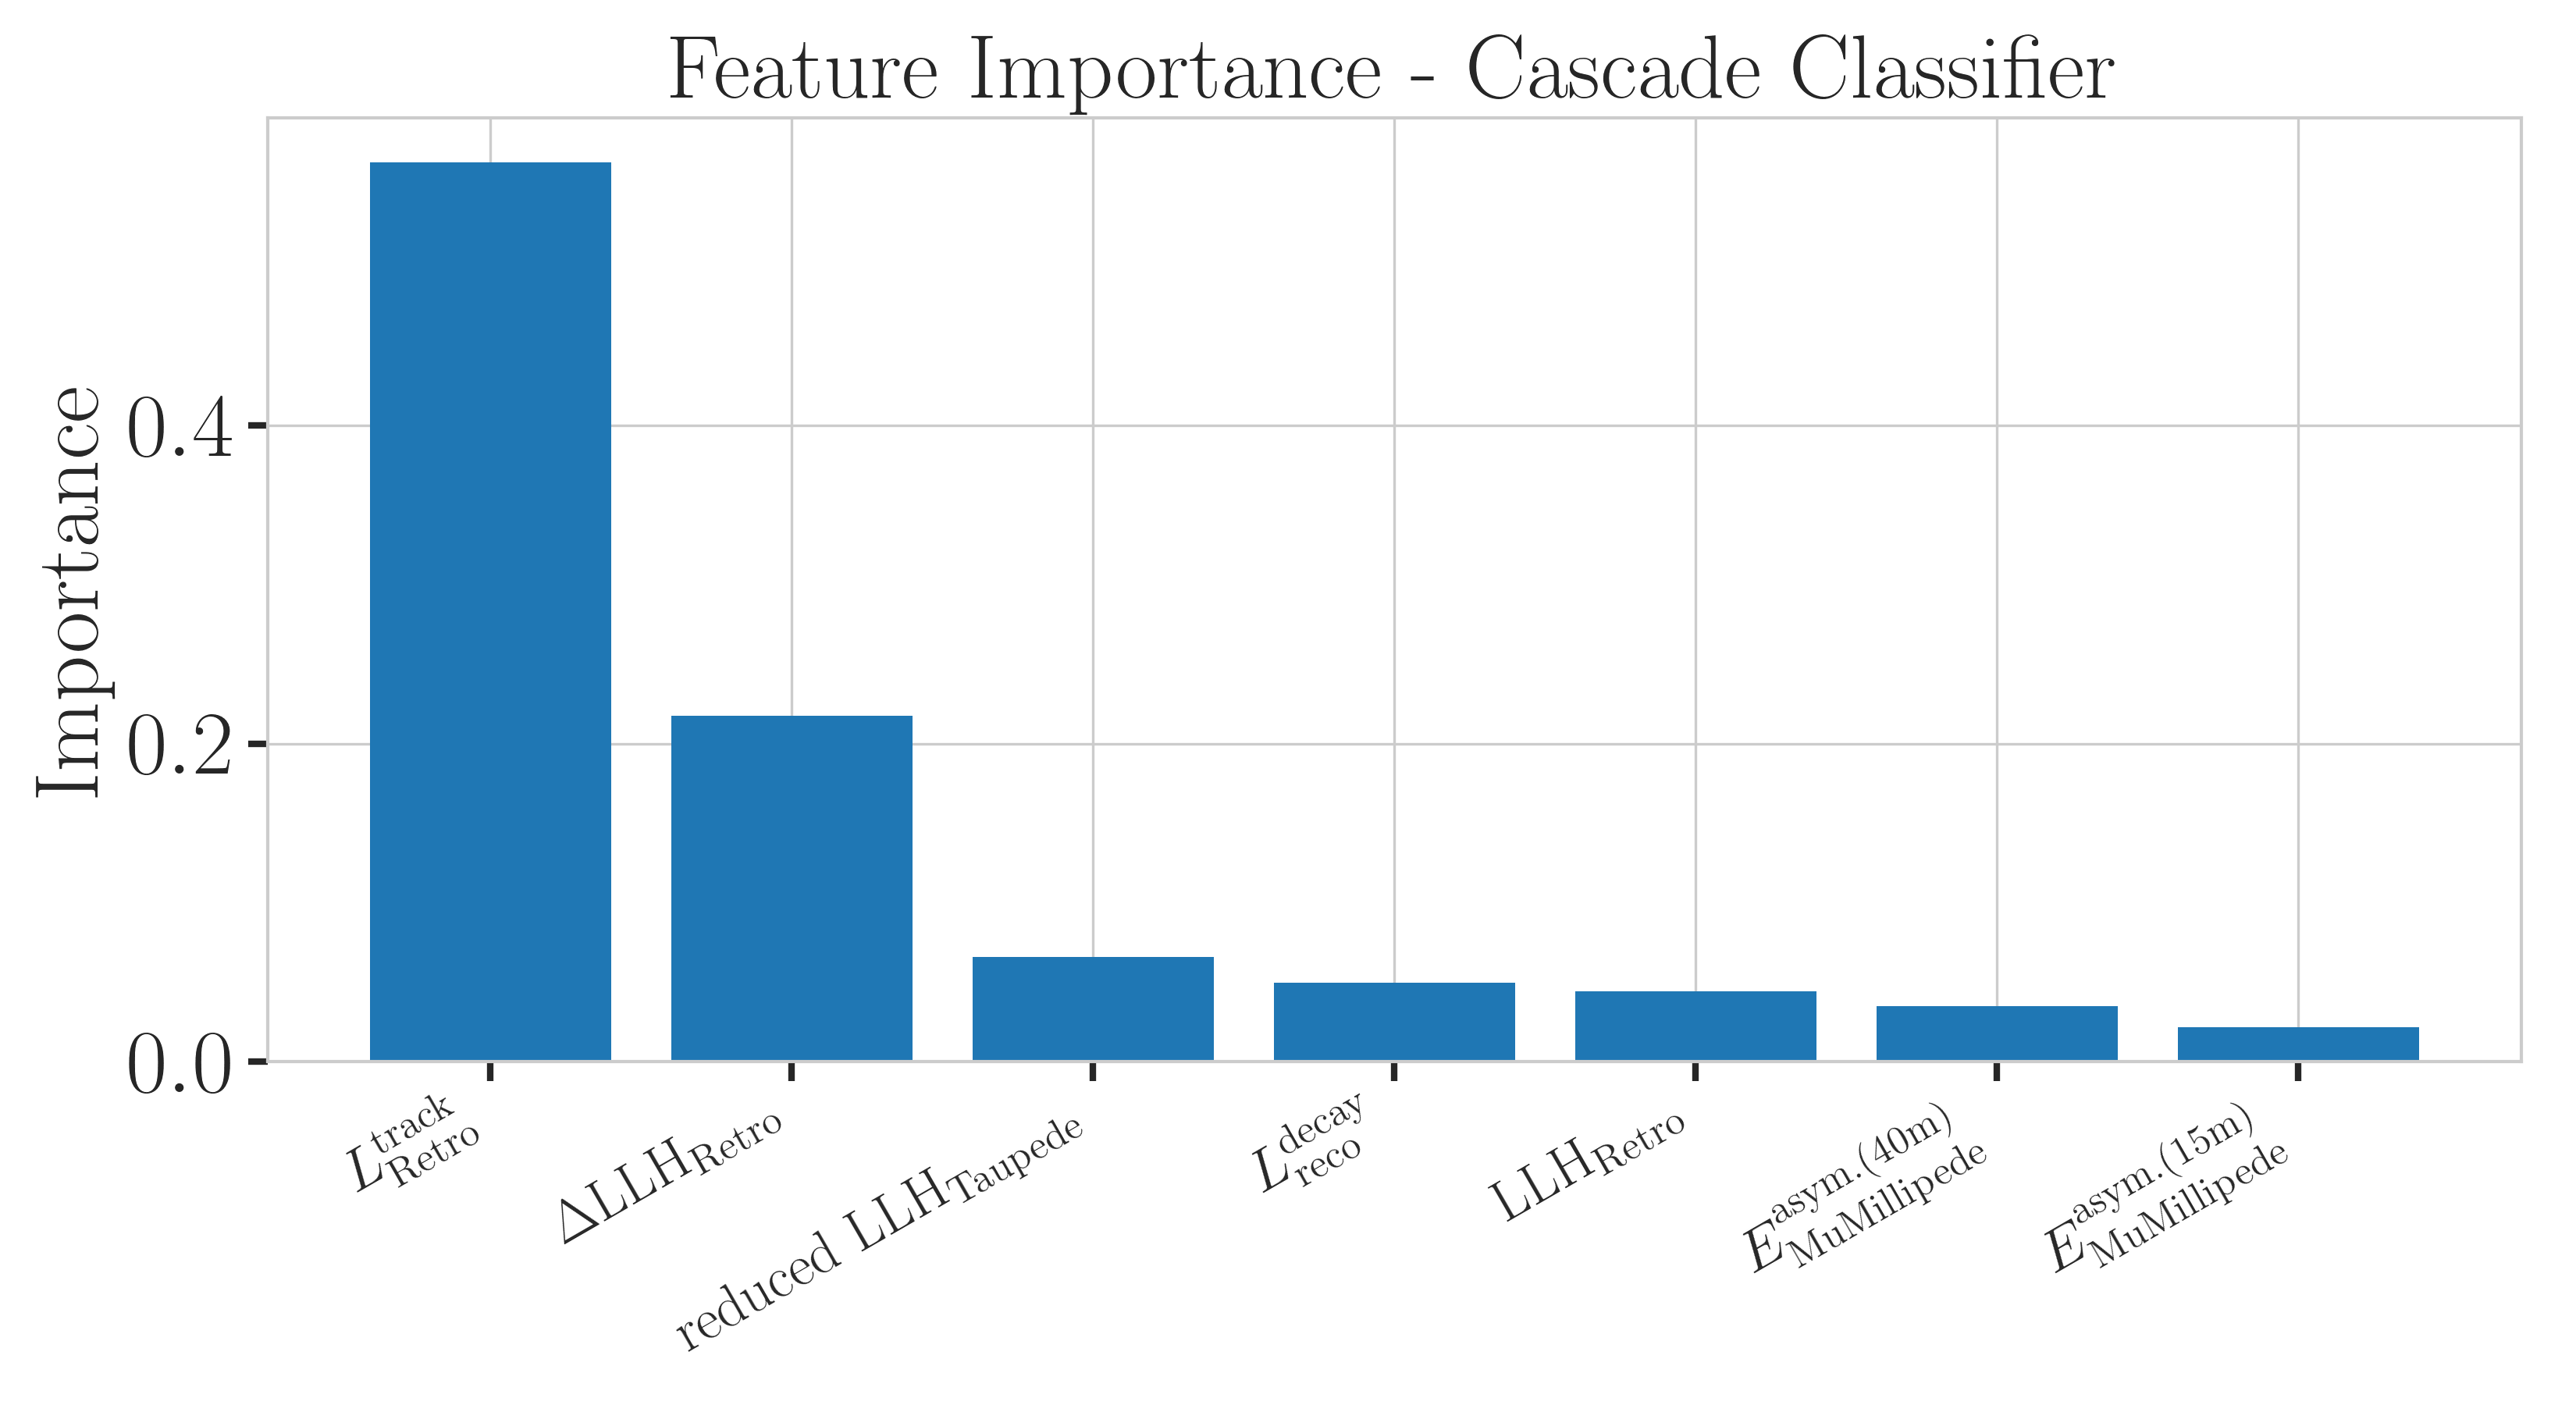
\includegraphics[width=0.8\linewidth]{figures/results/190607/classification/cascade_feature_importance.png}
    \caption[Double-cascade classifiers feature importances]{Feature importances of the  classifiers trained to distinguish double-cascades from tracks (top) and from cascades (bottom).}
    \labfig{track_classifier_features}
\end{figure*}


\section{FLERCNN Resolutions} \labsec{flercnn_resolutions_appendix}

\begin{figure}[h]
    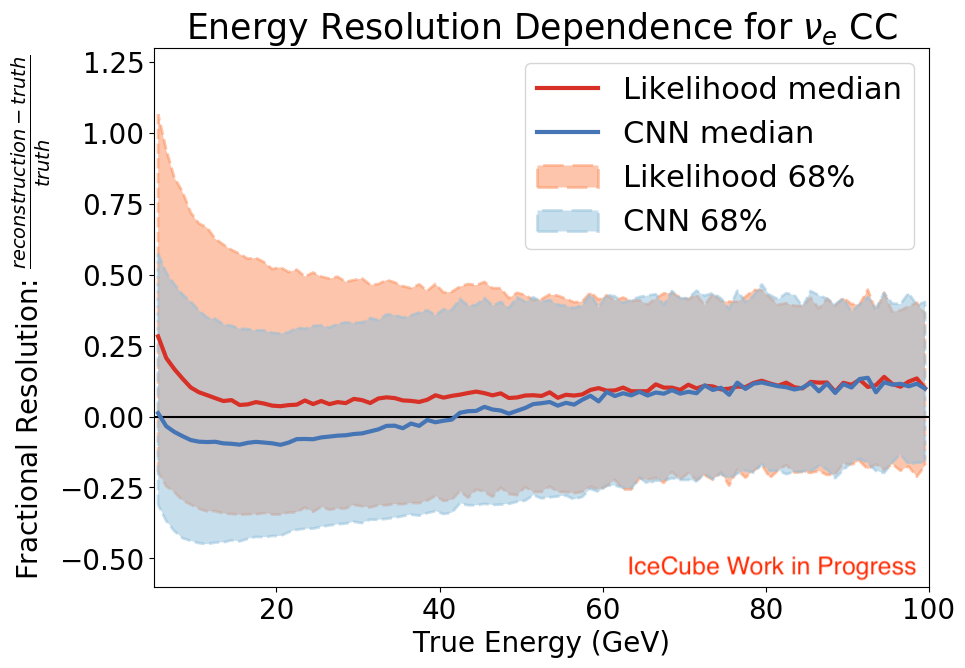
\includegraphics[width=0.8\textwidth]{figures/simulation_and_processing/flercnn/EnergyCNNResolution_NuECC_CompareLikelihoodReco.png}
	\caption[FLERCNN energy resolution for electron neutrinos]{Energy resolution of the FLERCNN reconstruction for electron neutrinos, compared to the performance of a classical, likelihood based reconstruction. Shown is the median fractional energy resolution and the \SI{68}{\percent} band as a function of the true energy.}
    \labfig{flercnn_resolution_example_appendix}
\end{figure}


\setchapterstyle{lines}
\chapter{Analysis Results}
\labch{analysis_results}

\section{Final Level Simulation Distributions} \labsec{final_level_simulation_appendix}

\begin{figure*}[h]
    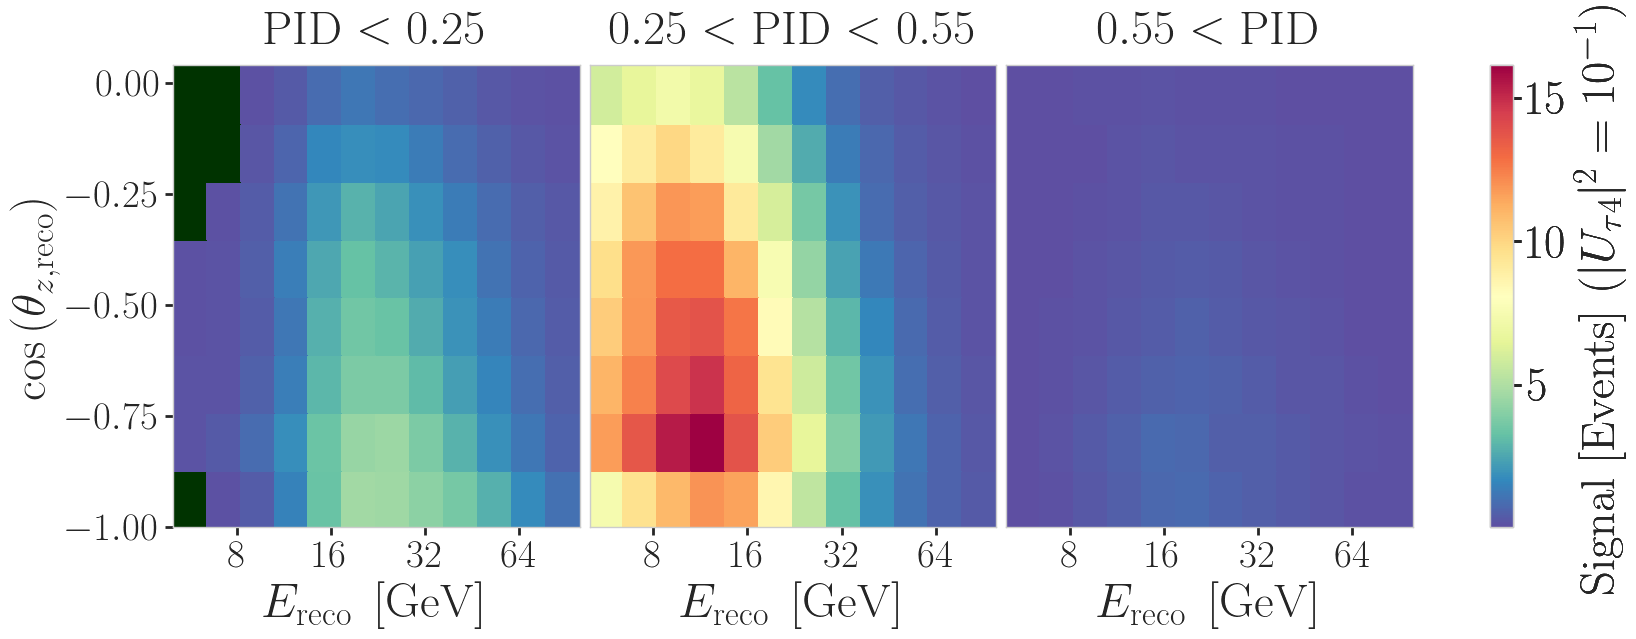
\includegraphics{figures/results/3d_histograms/signal_1.0_GeV_combined_U_tau4_sq_0.1000_total.png}
    \caption[Three-dimensional signal expectation]{Signal expectation in \SI{9.28}{years} for the \SI{1.0}{\gev} mass sample at a mixing of $0.1$, while all other parameters are at their nominal values (top) and observed data (bottom).}
    \labfig{signal_1.0_GeV_0.1_mixing}
\end{figure*}


\section{Treatment of Detector Systematic Uncertainties} \labsec{ultrasurfaces_appendix}

Shown is the performance of the detector systematic uncertainty treatment. The systematic set 0001 and 0004 have the DOM efficiency varied by $\pm10\%$, while set 0504 and 0505 have the ice absorption varied by $\pm10\%$. Set 0506 and 0507 have the ice scattering varied by $\pm10\%$, and set 1122 is the set with the new ice model, including the birefringence effect. The sets 0301, 0309, 190, 1901, 1902, and 1903 have variations of the hole ice p0 and p1 parameters, covering a wide range.

\begin{figure}[h]
    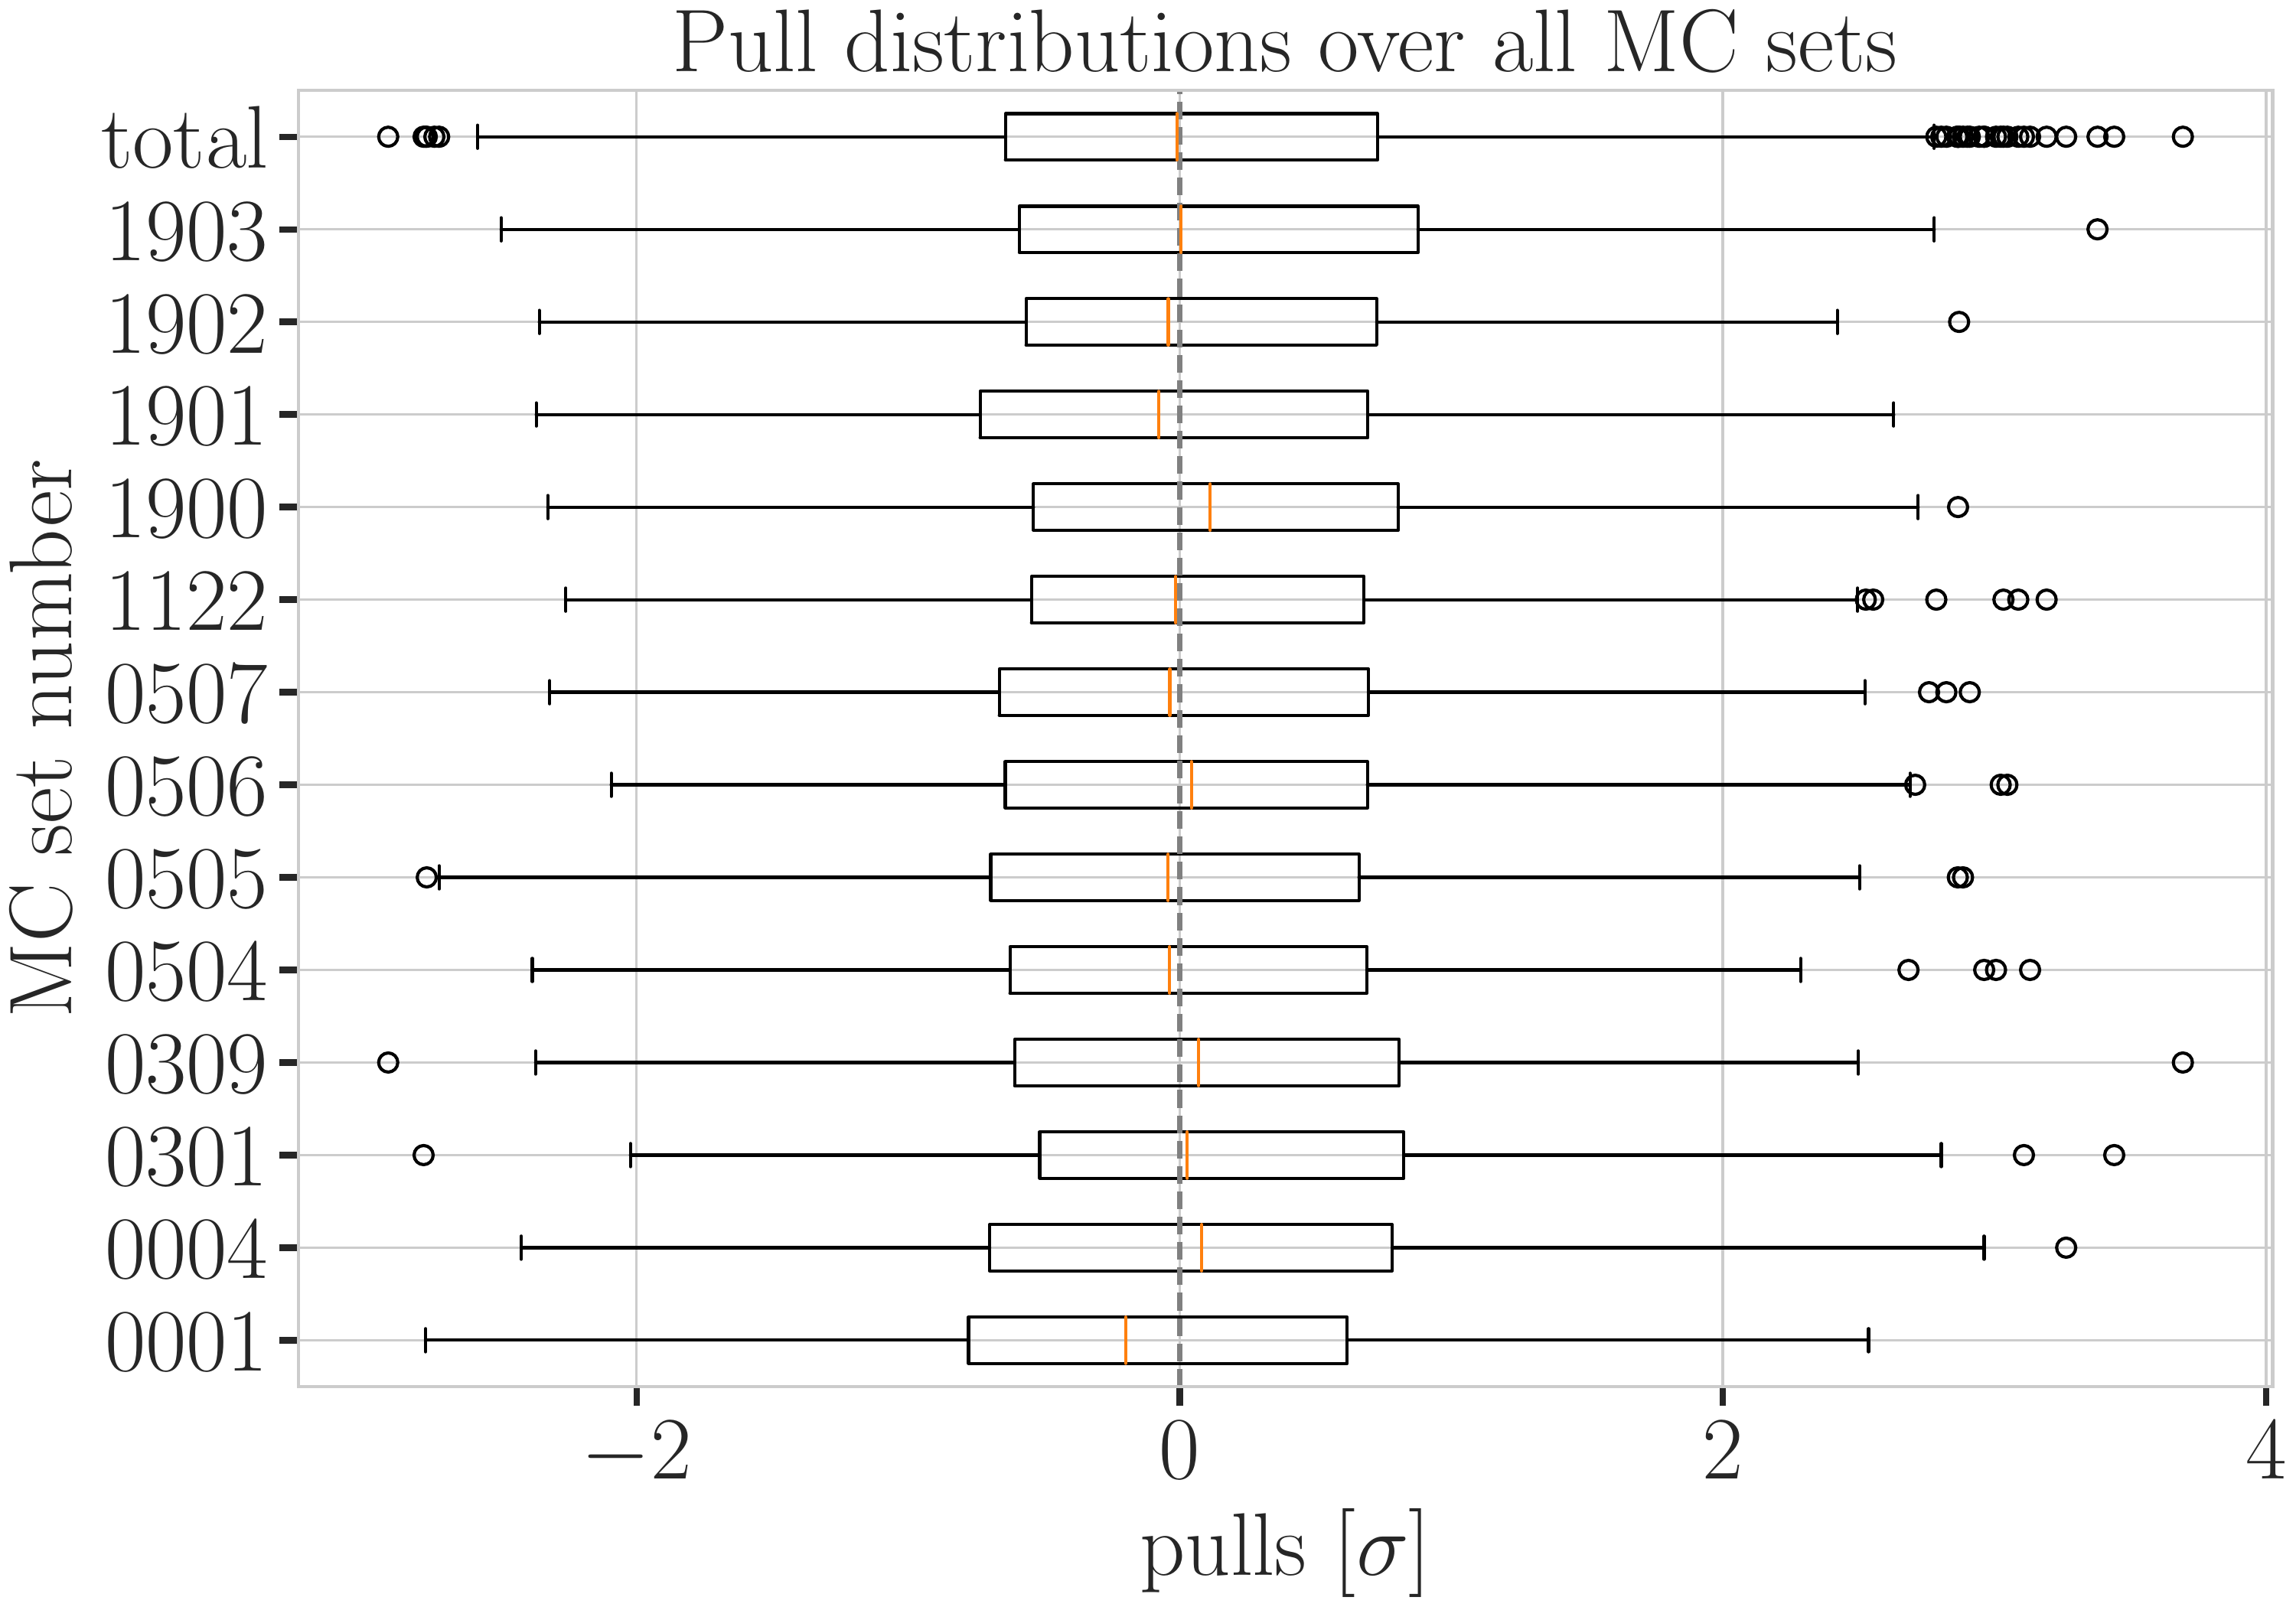
\includegraphics[width=0.9\textwidth]{figures/results/utlrasurfaces/oscNext_leptoninjector_1.0_GeV_knn_probs_neighbors_500_weighted_nfiles_extended_holeice_corrected_grads_poly_2_weighted_reference_weight_0.0100_thesis_style-2.png}
    \caption[Detector systematic uncertainty treatment overall performance]{Overall performance of the detector systematic uncertainty treatment. Shown are the pull distributions of the three-dimensional pulls shown in \reffig{hnl_ultrasurfaces_3d_pulls_selection0} and \reffig{hnl_ultrasurfaces_3d_pulls_selection1} between the nominal set and the specific systematic set, after the nominal set was re-weighted to the corresponding systematic parameter value.}
    \labfig{hnl_ultrasurfaces_all_pull_distributions}
\end{figure}

\begin{figure*}[h]
    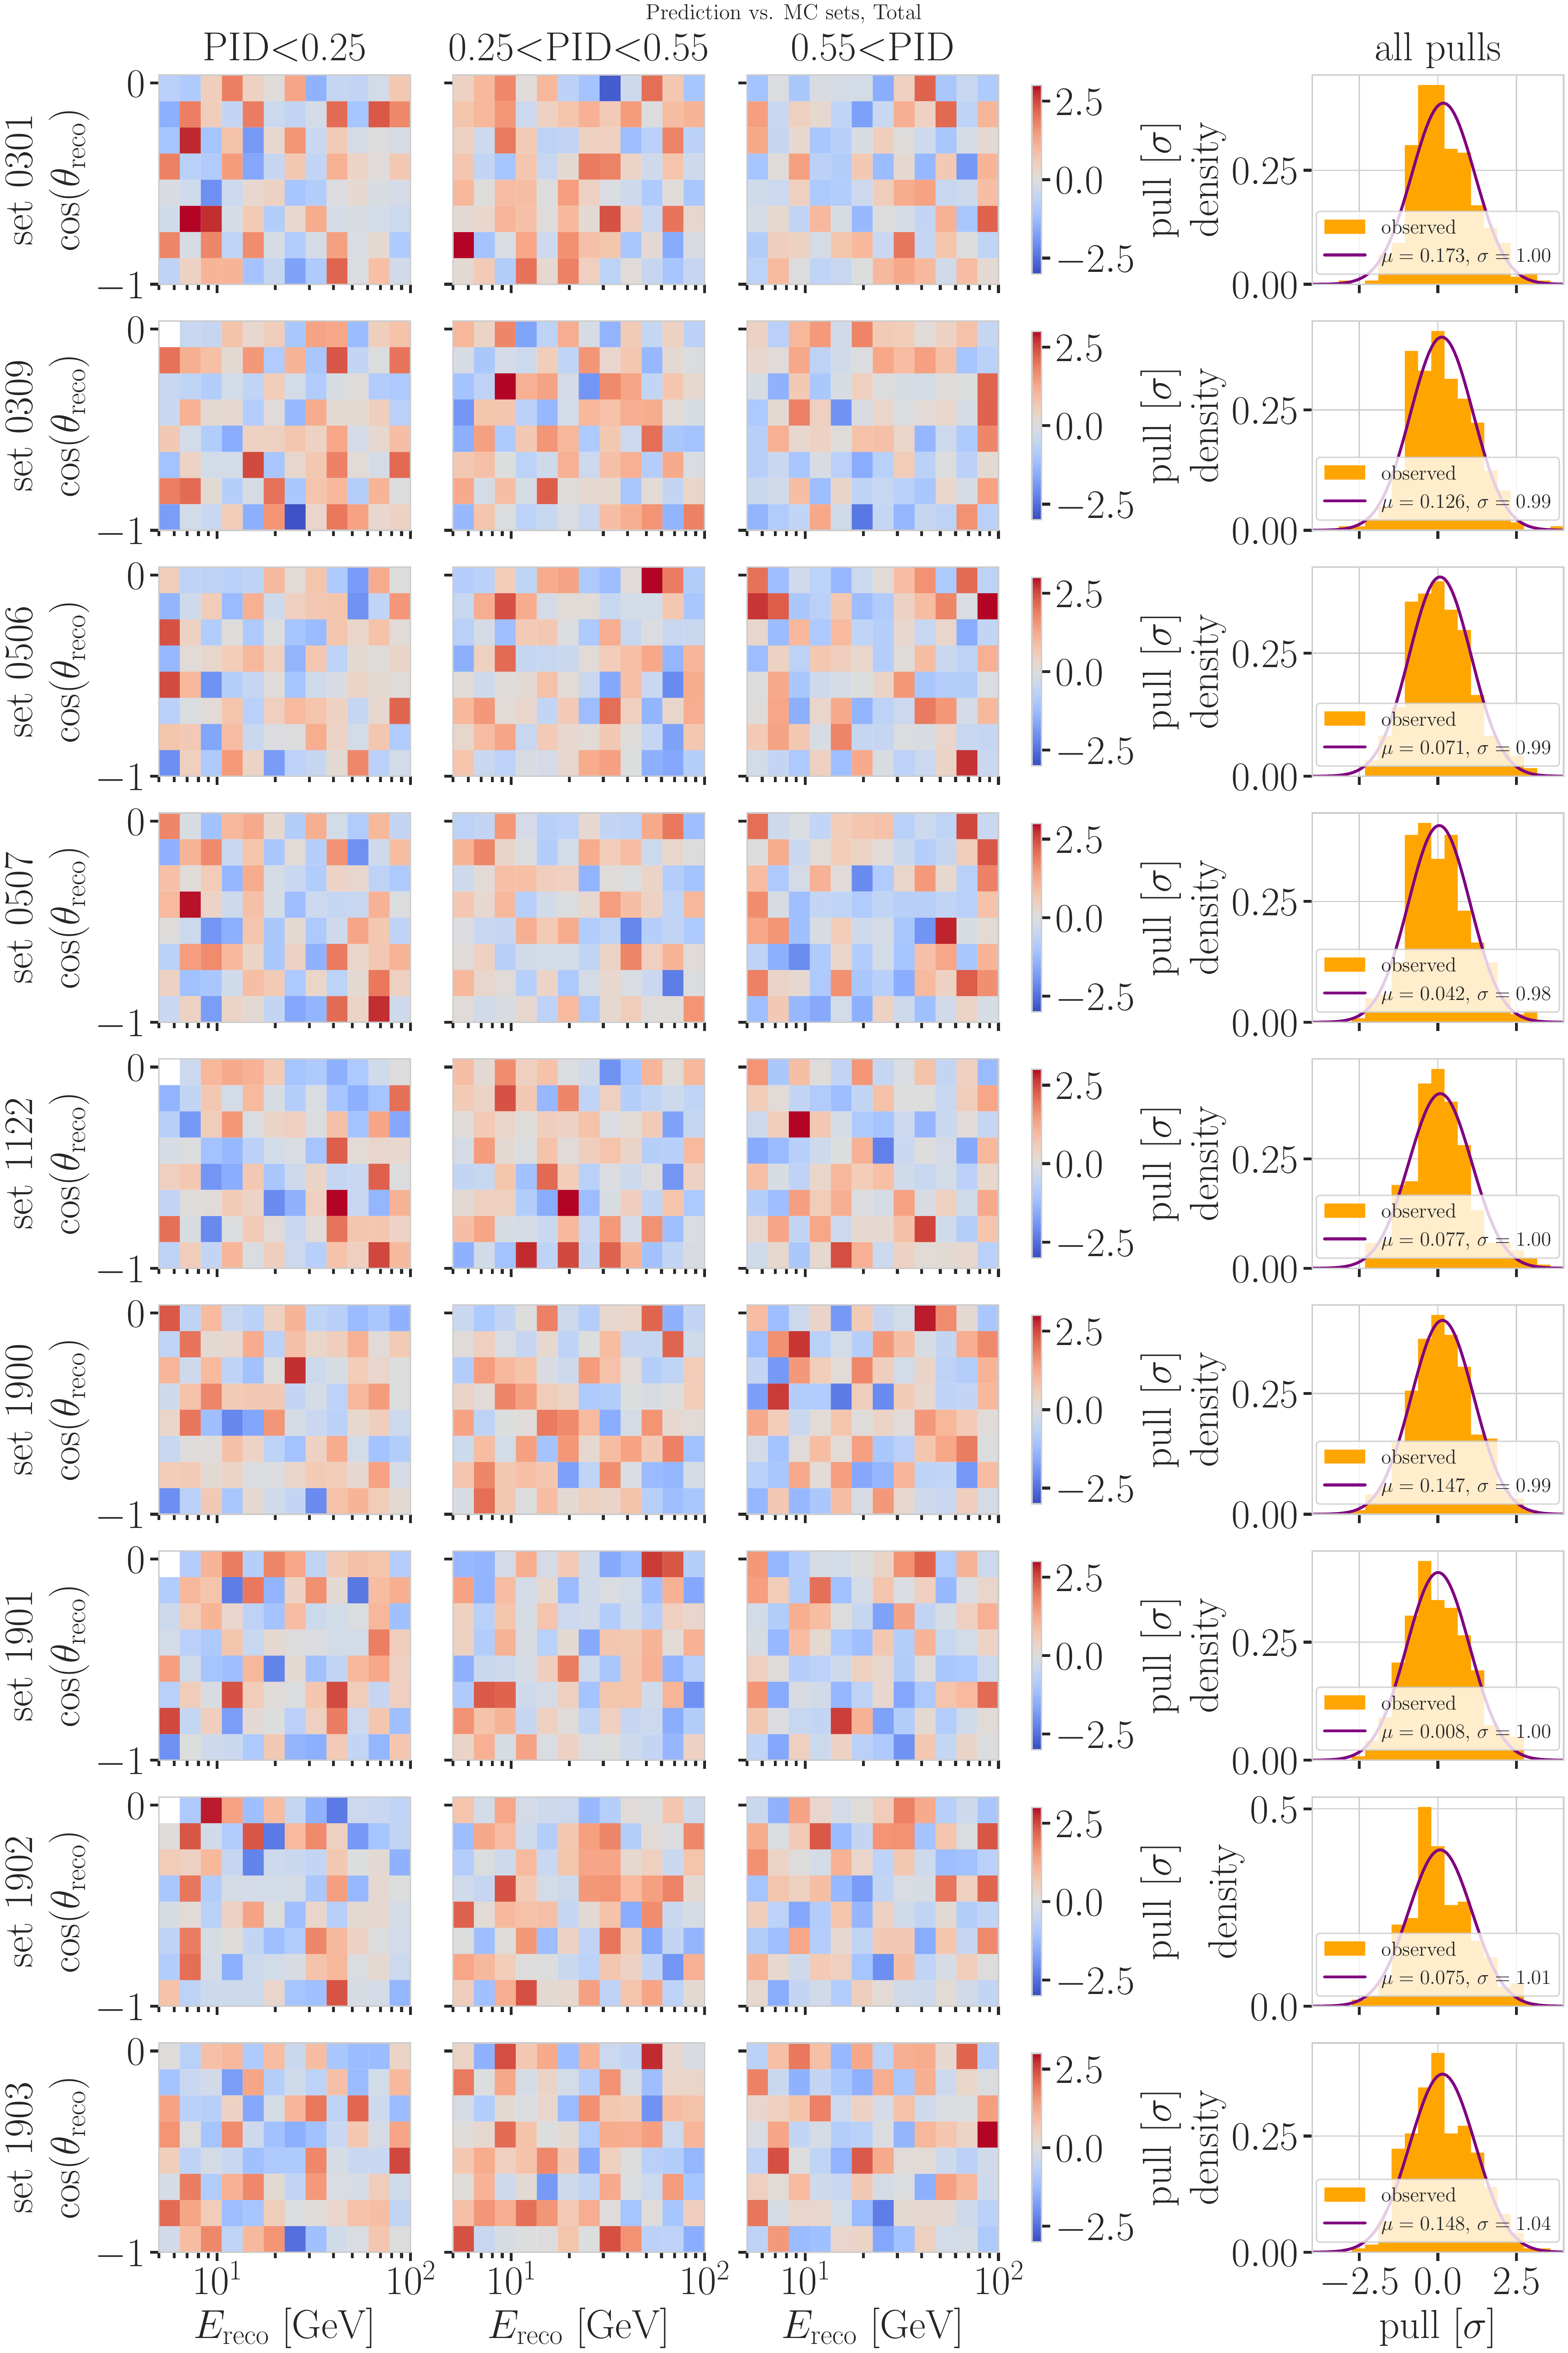
\includegraphics{figures/results/utlrasurfaces/oscNext_leptoninjector_1.0_GeV_knn_probs_neighbors_500_weighted_nfiles_extended_holeice_corrected_grads_poly_2_weighted_reference_weight_0.0100_thesis_style_subset_1-5.png}
    \caption[Detector systematic uncertainty treatment bin-wise pulls additional sets]{Three-dimensional pulls and set-wise pull distributions between the nominal set and the specific systematic sets, after the nominal set was re-weighted to the corresponding systematic parameter value.}
    \labfig{hnl_ultrasurfaces_3d_pulls_selection1}
\end{figure*}


\section{Data/MC Agreement} \labsec{data_mc_agreement_appendix}

\begin{figure*}[h]
    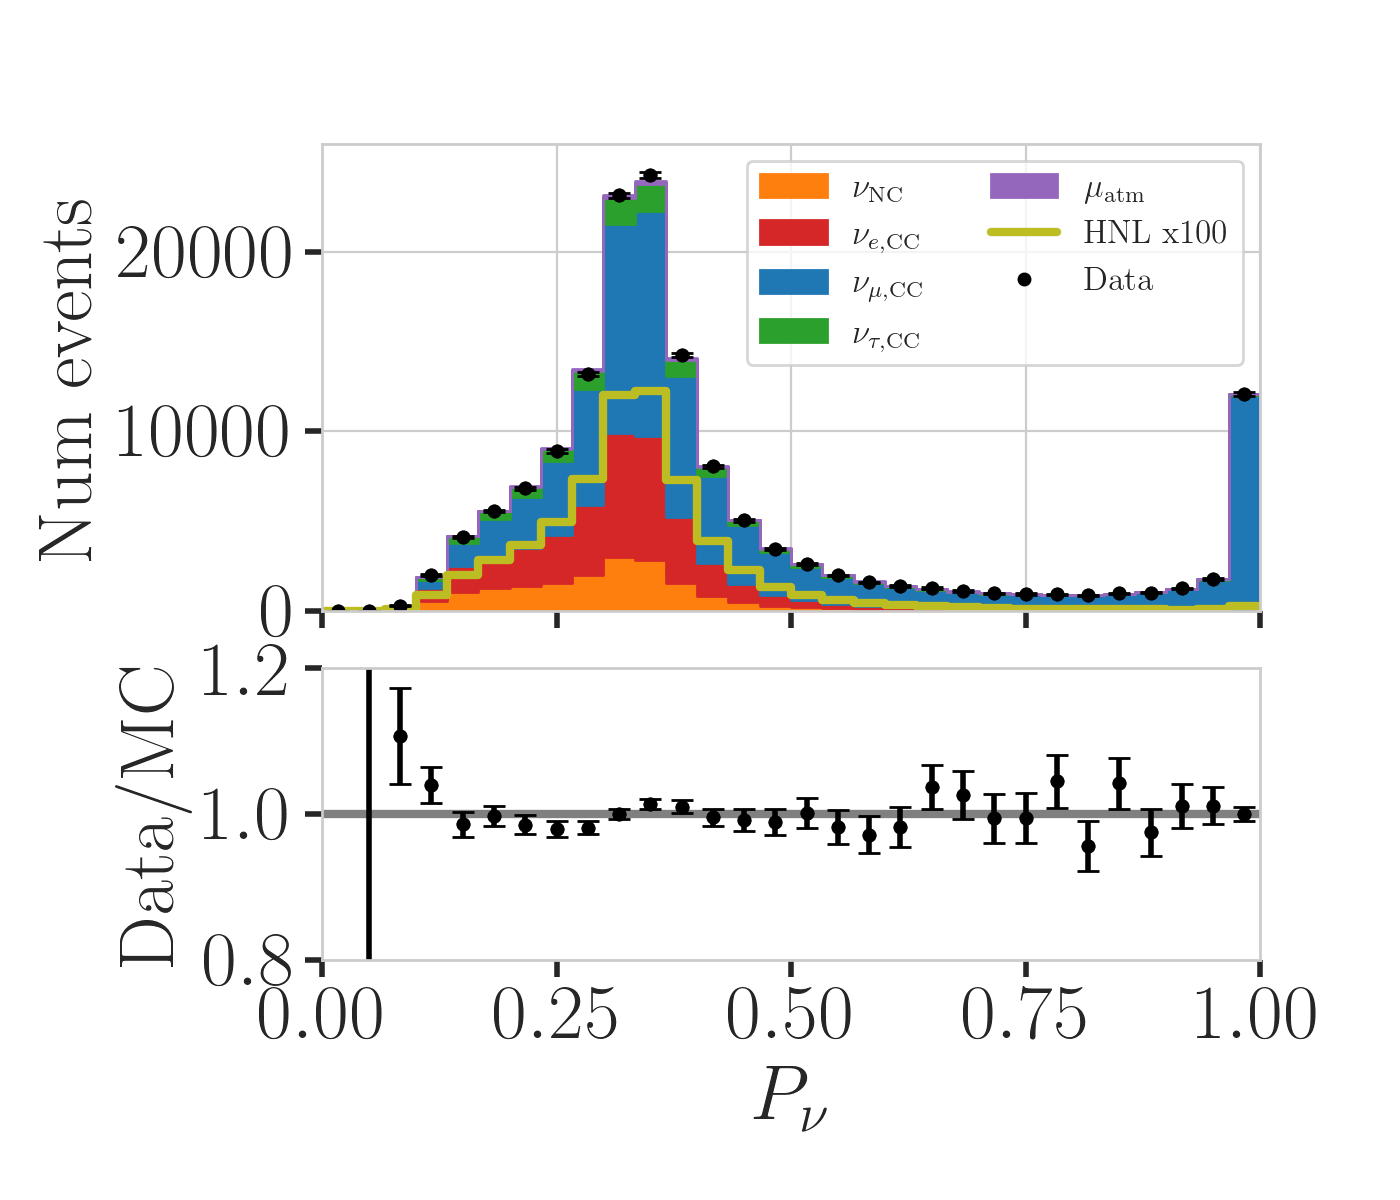
\includegraphics[width=0.49\linewidth]{figures/results/best_fit/pid_data_mc_agreement.png}
    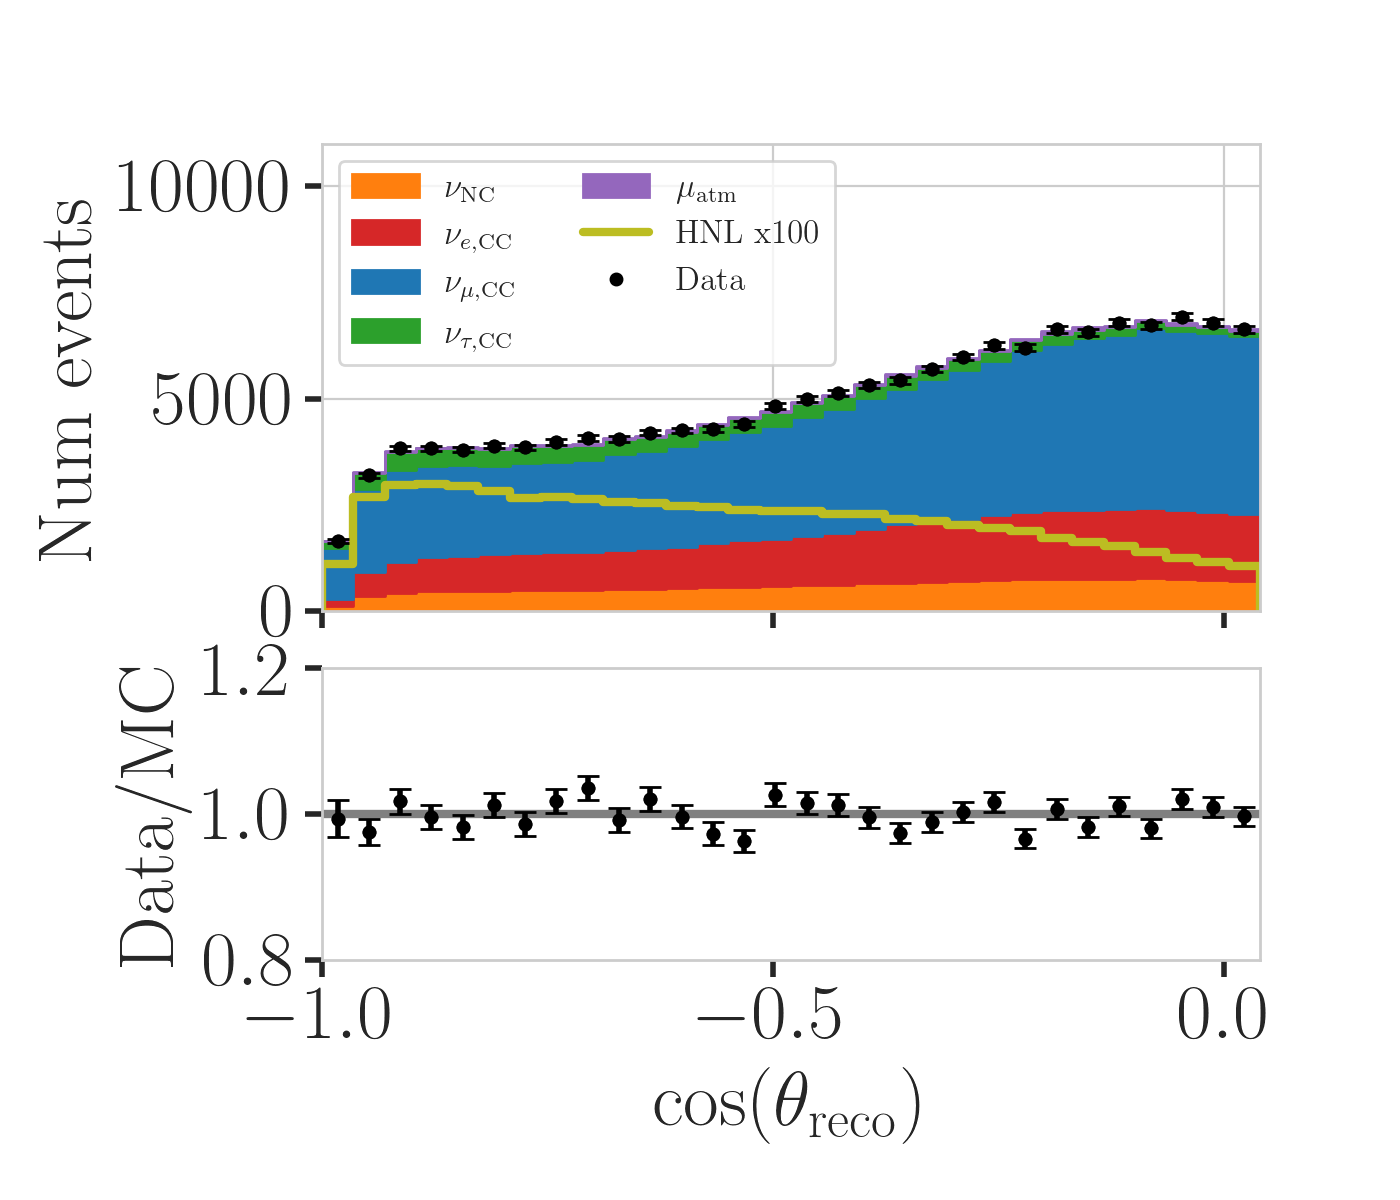
\includegraphics[width=0.49\linewidth]{figures/results/best_fit/reco_coszen_data_mc_agreement.png}
	\caption[PID and cosine of the zenith angle data/MC comparison]{Data/MC comparison of the PID (top) and cosine of the zenith angle (bottom) for the \SI{0.6}{\gev} mass sample. The data is compared to the total MC expectation, which is also split up into individual components for illustration. The HNL events are shown as part of the $\nu_\mathrm{NC}$ events in the stacked histogram, while 100x the HNL events are shown individually.}
    \labfig{1_d_data_mc_bfp_1.0_GeV_pid_cosz}
\end{figure*}


\section{Best Fit Nuisance Parameters}

\begin{table*}[h!]
    \begin{tabular}{ ll lll lll }
    \hline\hline
    \textbf{Parameter} & \textbf{Nominal} & \multicolumn{3}{c}{\textbf{Best Fit}} & \multicolumn{3}{c}{\textbf{Nominal - Best Fit}} \\ 
    & & \textbf{0.3 GeV} & \textbf{0.6 GeV} &  \textbf{1.0 GeV} & \textbf{0.3 GeV} & \textbf{0.6 GeV} &  \textbf{1.0 GeV} \\ 
    \hline\hline
    % $|U_{\tau 4}|^2$ & - & 0.003019 & 0.080494 & 0.106141 & - & - & - \\
    $\theta_{23} [\si{\degree}]$ & 47.5047 & 48.117185 & 47.918758 & 48.010986 & $-$0.612485 & $-$0.414058 & $-$0.506286 \\
    $\Delta m^{2}_{31} [\si{\electronvolt^2}]$ & 0.002475  & 0.002454  & 0.002454  & 0.002455  & 0.000020  & 0.000021  & 0.000019  \\
    \hline
    $N_{\nu}$ & 1.0  & 0.889149  & 0.889055  & 0.889559  & 0.110851  & 0.110945  & 0.110441  \\
    $\Delta \gamma_\nu$ & 0.0  & $-$0.007926 & $-$0.006692 & $-$0.006596 & 0.007926  & 0.006692  & 0.006596  \\
    $\rm{Barr} \; h_{\pi^+}$ & 0.0  & $-$0.147475 & $-$0.148481 & $-$0.148059 & 0.147475  & 0.148481  & 0.148059  \\
    $\rm{Barr} \; i_{\pi^+}$ & 0.0  & 0.475448  & 0.513393  & 0.521626  & $-$0.475448 & $-$0.513393 & $-$0.521626 \\
    $\rm{Barr} \; y_{K^+}$ & 0.0  & 0.076176  & 0.062893  & 0.057548  & $-$0.076176 & $-$0.062893 & $-$0.057548 \\
    \hline
    $\rm{DIS}$ & 0.0  & $-$0.248709 & $-$0.223302 & $-$0.215666 & 0.248709  & 0.223302  & 0.215666  \\
    $M_\rm{A,QE}$ & 0.0  & $-$0.170528 & $-$0.128150 & $-$0.120345 & 0.170528  & 0.128150  & 0.120345  \\
    $M_\rm{A,res}$ & 0.0  & $-$0.125855 & $-$0.080875 & $-$0.070716 & 0.125855  & 0.080875  & 0.070716  \\
    \hline
    $\epsilon_{\rm{DOM}}$ & 1.0  & 1.021984  & 1.017789  & 1.016689  & $-$0.021984 & $-$0.017789 & $-$0.016689 \\
    $\rm{hole \, ice} \; p_0$ & 0.101569  & $-$0.161341 & $-$0.161051 & $-$0.160129 & 0.262910  & 0.262620  & 0.261698  \\
    $\rm{hole \, ice} \; p_1$ & $-$0.049344 & $-$0.073701 & $-$0.075596 & $-$0.076261 & 0.024357  & 0.026252  & 0.026917  \\
    $\rm{ice \, absorption}$ & 1.00  & 0.943261  & 0.942463  & 0.942000  & 0.056739  & 0.057537  & 0.058000  \\
    $\rm{ice \, scattering}$ & 1.05  & 0.986152  & 0.989289  & 0.989438  & 0.063848  & 0.060711  & 0.060562  \\
    $N_\rm{bfr}$ & 0.0  & 0.746684  & 0.740255  & 0.736215  & $-$0.746684 & $-$0.740255 & $-$0.736215 \\
    \hline
    \end{tabular}
\caption[Best fit nuisance parameters values]{Best fit nuisance parameters for the three mass samples. Also shown is the nominal value and the difference between the nominal and the best fit.}
\labtab{best_fit_parameters}
\end{table*}
